\documentclass[../../General.tex]{subfiles}
\begin{document}

\section{Diseño de subsistema de elevación de piranómetro}\label{sec:subsistema_elevacion}

\subsection{Descripción general del subsistema}

El subsistema de elevación, mostrado en la Figura \ref{fig:SubsistemaPosicionamiento}, eleva el subsistema de orientación mediante un mecanismo de cuadrilátero articulado en paralelogramo. El plano del mecanismo contiene la dirección de avance del robot. Como el acoplador del paralelogramo se traslada sin rotar, la plataforma de orientación conserva su orientación respecto al chasis en todo el recorrido, y el subsistema de orientación solo debe corregir el alabeo. El mecanismo lleva el plano óptico de medición del piranómetro hasta una altura máxima de $1313.6\text{ mm}$ sobre el suelo, por encima de los $1300\text{ mm}$ definidos en la Tabla \ref{tab:lista_requerimientos}.

\begin{figure}[H]
	\captionsetup{justification=raggedright, singlelinecheck=false, labelsep=none}
	\caption[Vista isométrica y derecha del subsistema de elevación.]{}
	\textit{Vista isométrica y derecha del subsistema de elevación.} \par\medskip

	\begin{minipage}{0.5\textwidth}
		\centering
		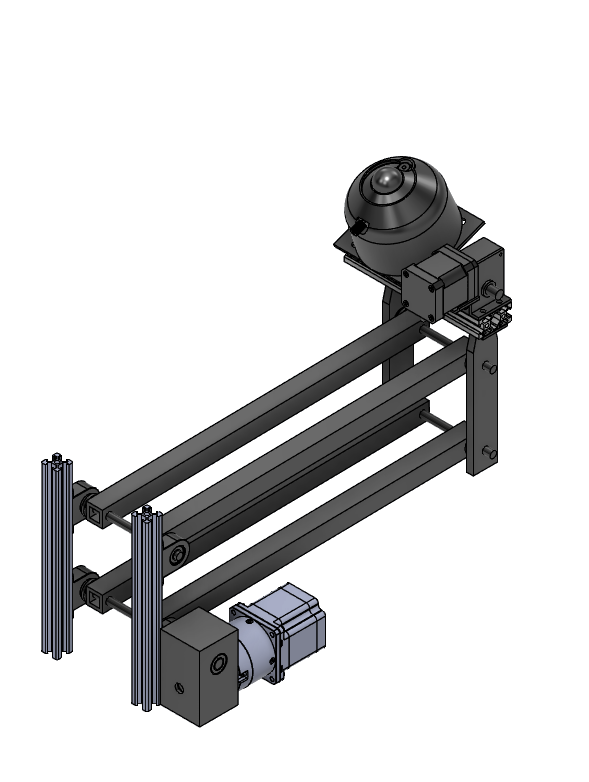
\includegraphics[width=\linewidth]{Recursos/Imagenes/ImagenesDisenoMecanico/MECANISMO_ELEVACION_ISO1.png}
	\end{minipage}\hfill
	\begin{minipage}{0.5\textwidth}
		\centering
		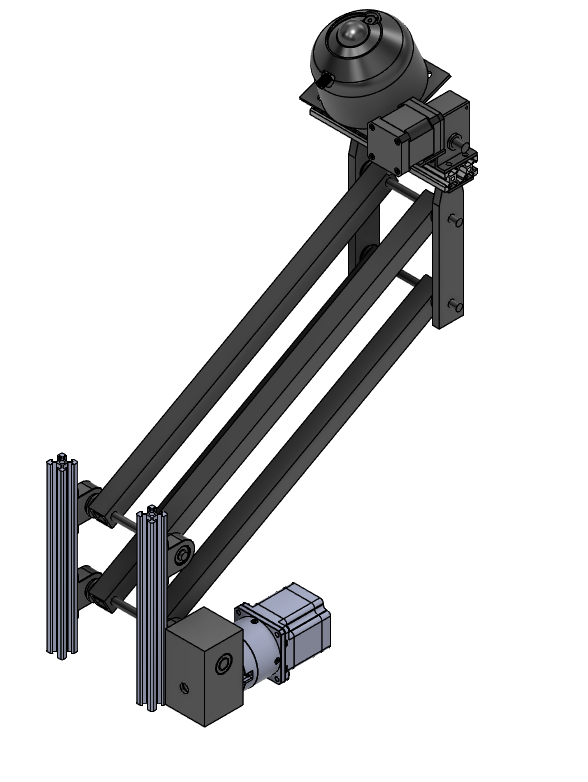
\includegraphics[width=\linewidth]{Recursos/Imagenes/ImagenesDisenoMecanico/MECANISMO_ELEVACION_ISO2.png}
	\end{minipage}
	\par\medskip

	\raggedright
	\footnotesize \textit{Nota.} Elaboración propia.
	\label{fig:SubsistemaPosicionamiento}
\end{figure}
% PENDIENTE: regenerar las figuras con L = 600 mm, A = 150 mm, w = 212 mm, el acoplador en U,
% los resortes, el motorreductor NMRVS40 + NEMA 34 y la estructura de la base definitiva.

El mecanismo está formado por cuatro brazos de tubo rectangular de aluminio 6061-T6 de $31.75 \times 25.40 \times 2.0\text{ mm}$, dispuestos en dos pares, uno a cada lado del plano medio. La distancia entre los pivotes de cada brazo es $L = 600\text{ mm}$ y la separación entre los dos pivotes de cada extremo es $A = 150\text{ mm}$. En la base, los pivotes se apoyan en una estructura de perfiles de aluminio 2020 unida al chasis. En el extremo superior, el acoplador es una sola pieza de chapa de aluminio 5052-H32 doblada en forma de U invertida: su alma sostiene la viga 2040 del subsistema de orientación y sus alas alojan los pivotes superiores. El ángulo de los brazos respecto a la horizontal varía entre $15^\circ$ y $70.3^\circ$. Este último valor deja una holgura de $6.69^\circ$ antes del ángulo en que los brazos superior e inferior entran en contacto ($77^\circ$).

Cada nodo se articula sobre un pasador de acero AISI 4140 rectificado de $\varnothing 8\text{ mm}$ (h6) con los extremos roscados, que se fija con perillas roscadas. Una tuerca y una arandela fijan la posición axial de cada brazo (en el lado accionado del pivote superior de la base, un separador), y cada brazo gira sobre una chumacera de brida KFL08 con carcasa de aleación de zinc, atornillada a la cara interior del tubo. La anchura interior entre las alas del acoplador, igual a la separación entre los brazos de la base, es de $212\text{ mm}$; la fija el espacio que ocupan los resortes de compensación en el pivote inferior.

El accionamiento se ubica en el pivote inferior, en el lado posterior del robot. Un motorreductor de tornillo sin fin, formado por un reductor NMRVS40 de relación 50:1 y un motor paso a paso NEMA 34, transmite el torque a uno de los brazos inferiores mediante un eje escalonado con chaveta y una brida atornillada al tubo. El reductor es autobloqueante en reposo, de modo que el mecanismo conserva su posición sin que el motor tenga que vencer la carga. Los dos brazos inferiores están unidos por un travesaño y cuatro cartelas (\textit{gusset plates}) y forman un solo marco rígido, por lo que el torque se reparte entre ambos lados y el mecanismo resiste las cargas laterales. Los brazos superiores no llevan cartelas. Dos resortes de torsión, uno por lado, compensan parte del momento gravitacional y reducen el torque que debe entregar el motorreductor.

La posición angular de los brazos se mide con un sensor inercial MPU-6050 montado en uno de los brazos inferiores, que cierra el lazo de control de altura y permite detectar atascos. Como este sensor mide el ángulo del brazo respecto a la horizontal, su lectura incluye el cabeceo del chasis. El subsistema no corrige el cabeceo; por ello, la medición de irradiancia se realiza con el robot detenido y solo en tramos casi planos, cuya pendiente se verifica con el sensor inercial del eje basculante del subsistema de orientación.

\subsection{Planteamiento inicial y parámetros de diseño}

El subsistema debe llevar el plano óptico del piranómetro hasta $1300\text{ mm}$ sobre el suelo y ajustar su altura en cada punto de medición con una tolerancia de $\pm 15\text{ mm}$. El robot se detiene, ajusta la altura y mide. Los datos de entrada y las restricciones del análisis se resumen en la Tabla \ref{tab:parametros_diseno_elev}.

\begin{center}
    \footnotesize
    \begin{xltabular}{\textwidth}{|p{3.5cm}|>{\centering\arraybackslash}p{2.2cm}|>{\centering\arraybackslash}p{2.8cm}|>{\centering\arraybackslash}X|}
        \caption{Datos de entrada y restricciones del subsistema de elevación\label{tab:parametros_diseno_elev}} \\
        \hline
        \rowcolor[HTML]{D9E1F2}
        Parámetro & Símbolo & Valor & Descripción \\ \hline
        \endfirsthead

        \multicolumn{4}{c}%
        {\tablename\ \thetable{} -- Continuación de la página anterior} \\
        \hline
        \rowcolor[HTML]{D9E1F2}
        Parámetro & Símbolo & Valor & Descripción \\ \hline
        \endhead

        \hline
        \endfoot

        \hline
        \endlastfoot

        \multicolumn{4}{|l|}{\textbf{Geometría}} \\ \hline
        Distancia entre pivotes del brazo & $L$ & $600\text{ mm}$ & Longitud de corte del tubo: $650\text{ mm}$ ($25\text{ mm}$ de voladizo en cada extremo). \\ \hline
        Separación entre pivotes & $A$ & $150\text{ mm}$ & Igual en el acoplador y en la base. \\ \hline
        Sección de los brazos & -- & $31.75 \times 25.40 \times 2.0\text{ mm}$ & Tubo rectangular de aluminio 6061-T6; la dimensión mayor está en el plano del mecanismo. \\ \hline
        Ángulo mínimo & $\theta_{\text{mín}}$ & $15^\circ$ & Posición baja de los brazos respecto a la horizontal. \\ \hline
        Holgura angular & $\Delta\theta_{h}$ & $6.69^\circ$ & Margen antes del contacto entre brazos, que ocurre en $77^\circ$ (modelo CAD). \\ \hline
        Altura del pivote actuado & $z_p$ & $419.7\text{ mm}$ & Sobre el suelo (modelo CAD). \\ \hline
        Pivote superior a plano óptico & $z_c$ & $179\text{ mm}$ & $43\text{ mm}$ del pivote al alma y $136\text{ mm}$ de la cara inferior de la viga 2040 al plano óptico. \\ \hline
        Ancho interior del acoplador & $w$ & $212\text{ mm}$ & Distancia entre las caras interiores de las alas (Sección \ref{subsubsec:acoplador_elev}). \\ \hline
        \multicolumn{4}{|l|}{\textbf{Masas}} \\ \hline
        Subsistema de orientación & $m_{\text{blk}}$ & $1.890\text{ kg}$ & Incluye un piranómetro de $0.50\text{ kg}$ (modelo CAD). \\ \hline
        Acoplador en U & $m_{U}$ & $0.174\text{ kg}$ & Chapa de 5052-H32 de $3\text{ mm}$. \\ \hline
        Herrajes del acoplador & $m_{h}$ & $0.358\text{ kg}$ & Dos pasadores de $\varnothing 8 \times 242\text{ mm}$ (masa calculada), chumaceras, tornillería y perillas de los nodos superiores (modelo CAD). \\ \hline
        Masa de cada brazo & $m_{b}$ & $0.373\text{ kg}$ & Tubo de $650\text{ mm}$ con $0.574\text{ kg/m}$ \citep{aluminum2005manual}. \\ \hline
        \multicolumn{4}{|l|}{\textbf{Movimiento}} \\ \hline
        Tiempo de barrido & $t_{b}$ & $10\text{ s}$ & Tiempo para recorrer el barrido completo. \\ \hline
        Fracción de aceleración & $f_{a}$ & $0.25$ & Fracción de $t_b$ en aceleración e igual en desaceleración. \\ \hline
        Tolerancia de altura & $\Delta H$ & $\pm 15\text{ mm}$ & Error admisible del plano óptico respecto a la altura objetivo. \\ \hline
        \multicolumn{4}{|l|}{\textbf{Cargas de servicio}} \\ \hline
        Pendiente longitudinal & $\varphi$ & $\pm 16^\circ$ & Pendiente máxima del camino (Tabla \ref{tab:lista_requerimientos}). \\ \hline
        Velocidad de diseño del viento & $V$ & $75\text{ km/h}$ & Valor mínimo normativo \citep{nte_e020}. \\ \hline
        Factor de forma & $C$ & $1.5$ & Elementos con una dimensión corta en la dirección del viento. \\ \hline
        Factor de ráfaga & $f_r$ & $1.2$ & Estructura Tipo 2. \\ \hline
        Área lateral del subsistema de orientación & $A_{\text{lat}}$ & $0.012\text{ m}^2$ & Igual a la de la sección de orientación. \\ \hline
        Área frontal del subsistema de orientación & $A_{\text{fr}}$ & $0.008\text{ m}^2$ & Proyección en la dirección de avance (modelo CAD). \\ \hline
        \multicolumn{4}{|l|}{\textbf{Criterios}} \\ \hline
        Factor de servicio del actuador & $S$ & $1.30$ & Mismo criterio que en el subsistema de orientación. \\ \hline
    \end{xltabular}
\end{center}

La masa del subsistema de orientación se toma del modelo CAD e incluye la envolvente de $0.50\text{ kg}$ adoptada para el piranómetro. El análisis se basa en las siguientes hipótesis:
\begin{itemize}
    \item los eslabones, el acoplador y la base se comportan como cuerpos rígidos;
    \item las cargas son cuasiestáticas: no se consideran impactos por irregularidades del terreno ni las cargas de inercia por aceleración o frenado del robot, que se tratan en el subsistema de locomoción;
    \item el viento se evalúa con la velocidad mínima normativa a $10\text{ m}$ de altura, sin reducción por la menor altura del mecanismo, y actúa sobre el área completa de los cuatro brazos, sin descontar el apantallamiento entre ellos;
    \item la gravedad, el viento y la pendiente se combinan en su valor más desfavorable;
    \item el centro de masa del subsistema de orientación se ubica sobre la línea de pivotes del acoplador y en el plano medio del mecanismo.
\end{itemize}

\subsection{Planteamiento cinemático y estático}

\begin{figure}[H]
	\captionsetup{justification=raggedright, singlelinecheck=false, labelsep=none}
	\caption[Esquematización de movimiento del subsistema de elevación y diagrama de cuerpo libre.]{}
	\textit{Esquematización de movimiento del subsistema de elevación (izquierda) y diagrama de cuerpo libre (derecha).} \par\medskip

	\begin{minipage}{0.5\textwidth}
		\centering
		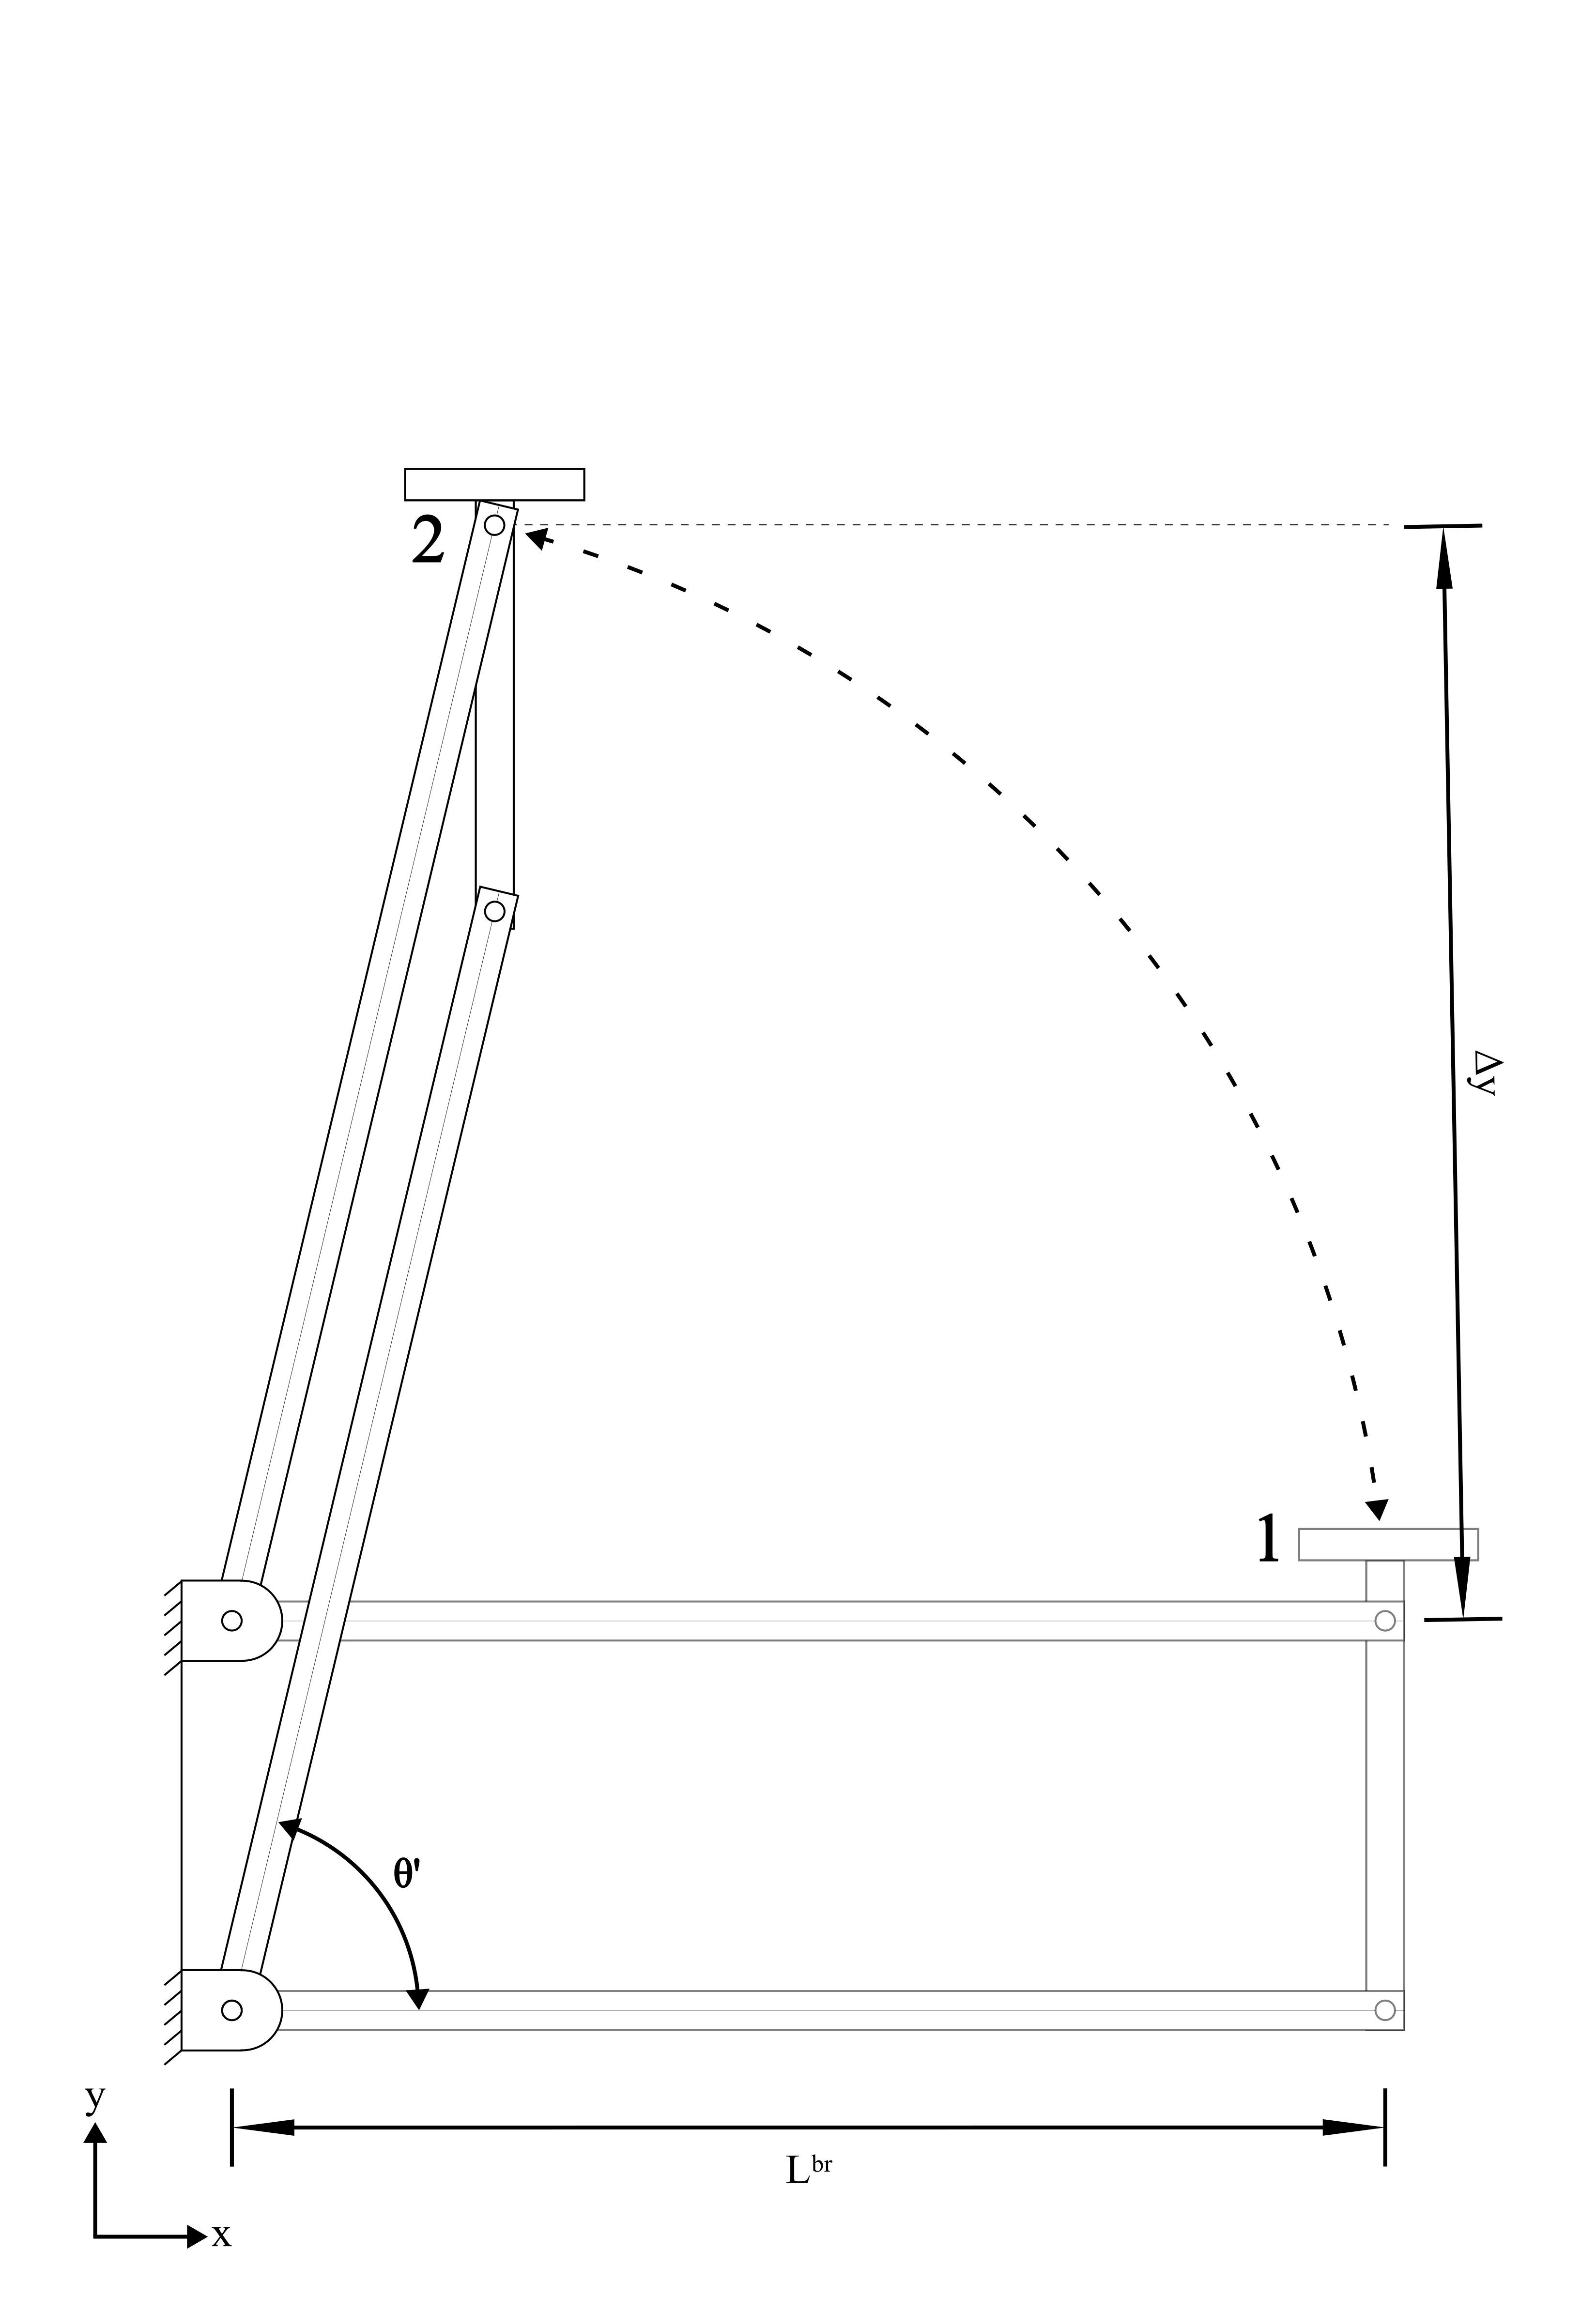
\includegraphics[width=\linewidth]{Recursos/Imagenes/ImagenesDisenoMecanico/4Bar_DCL_1.png}
	\end{minipage}\hfill
	\begin{minipage}{0.5\textwidth}
		\centering
		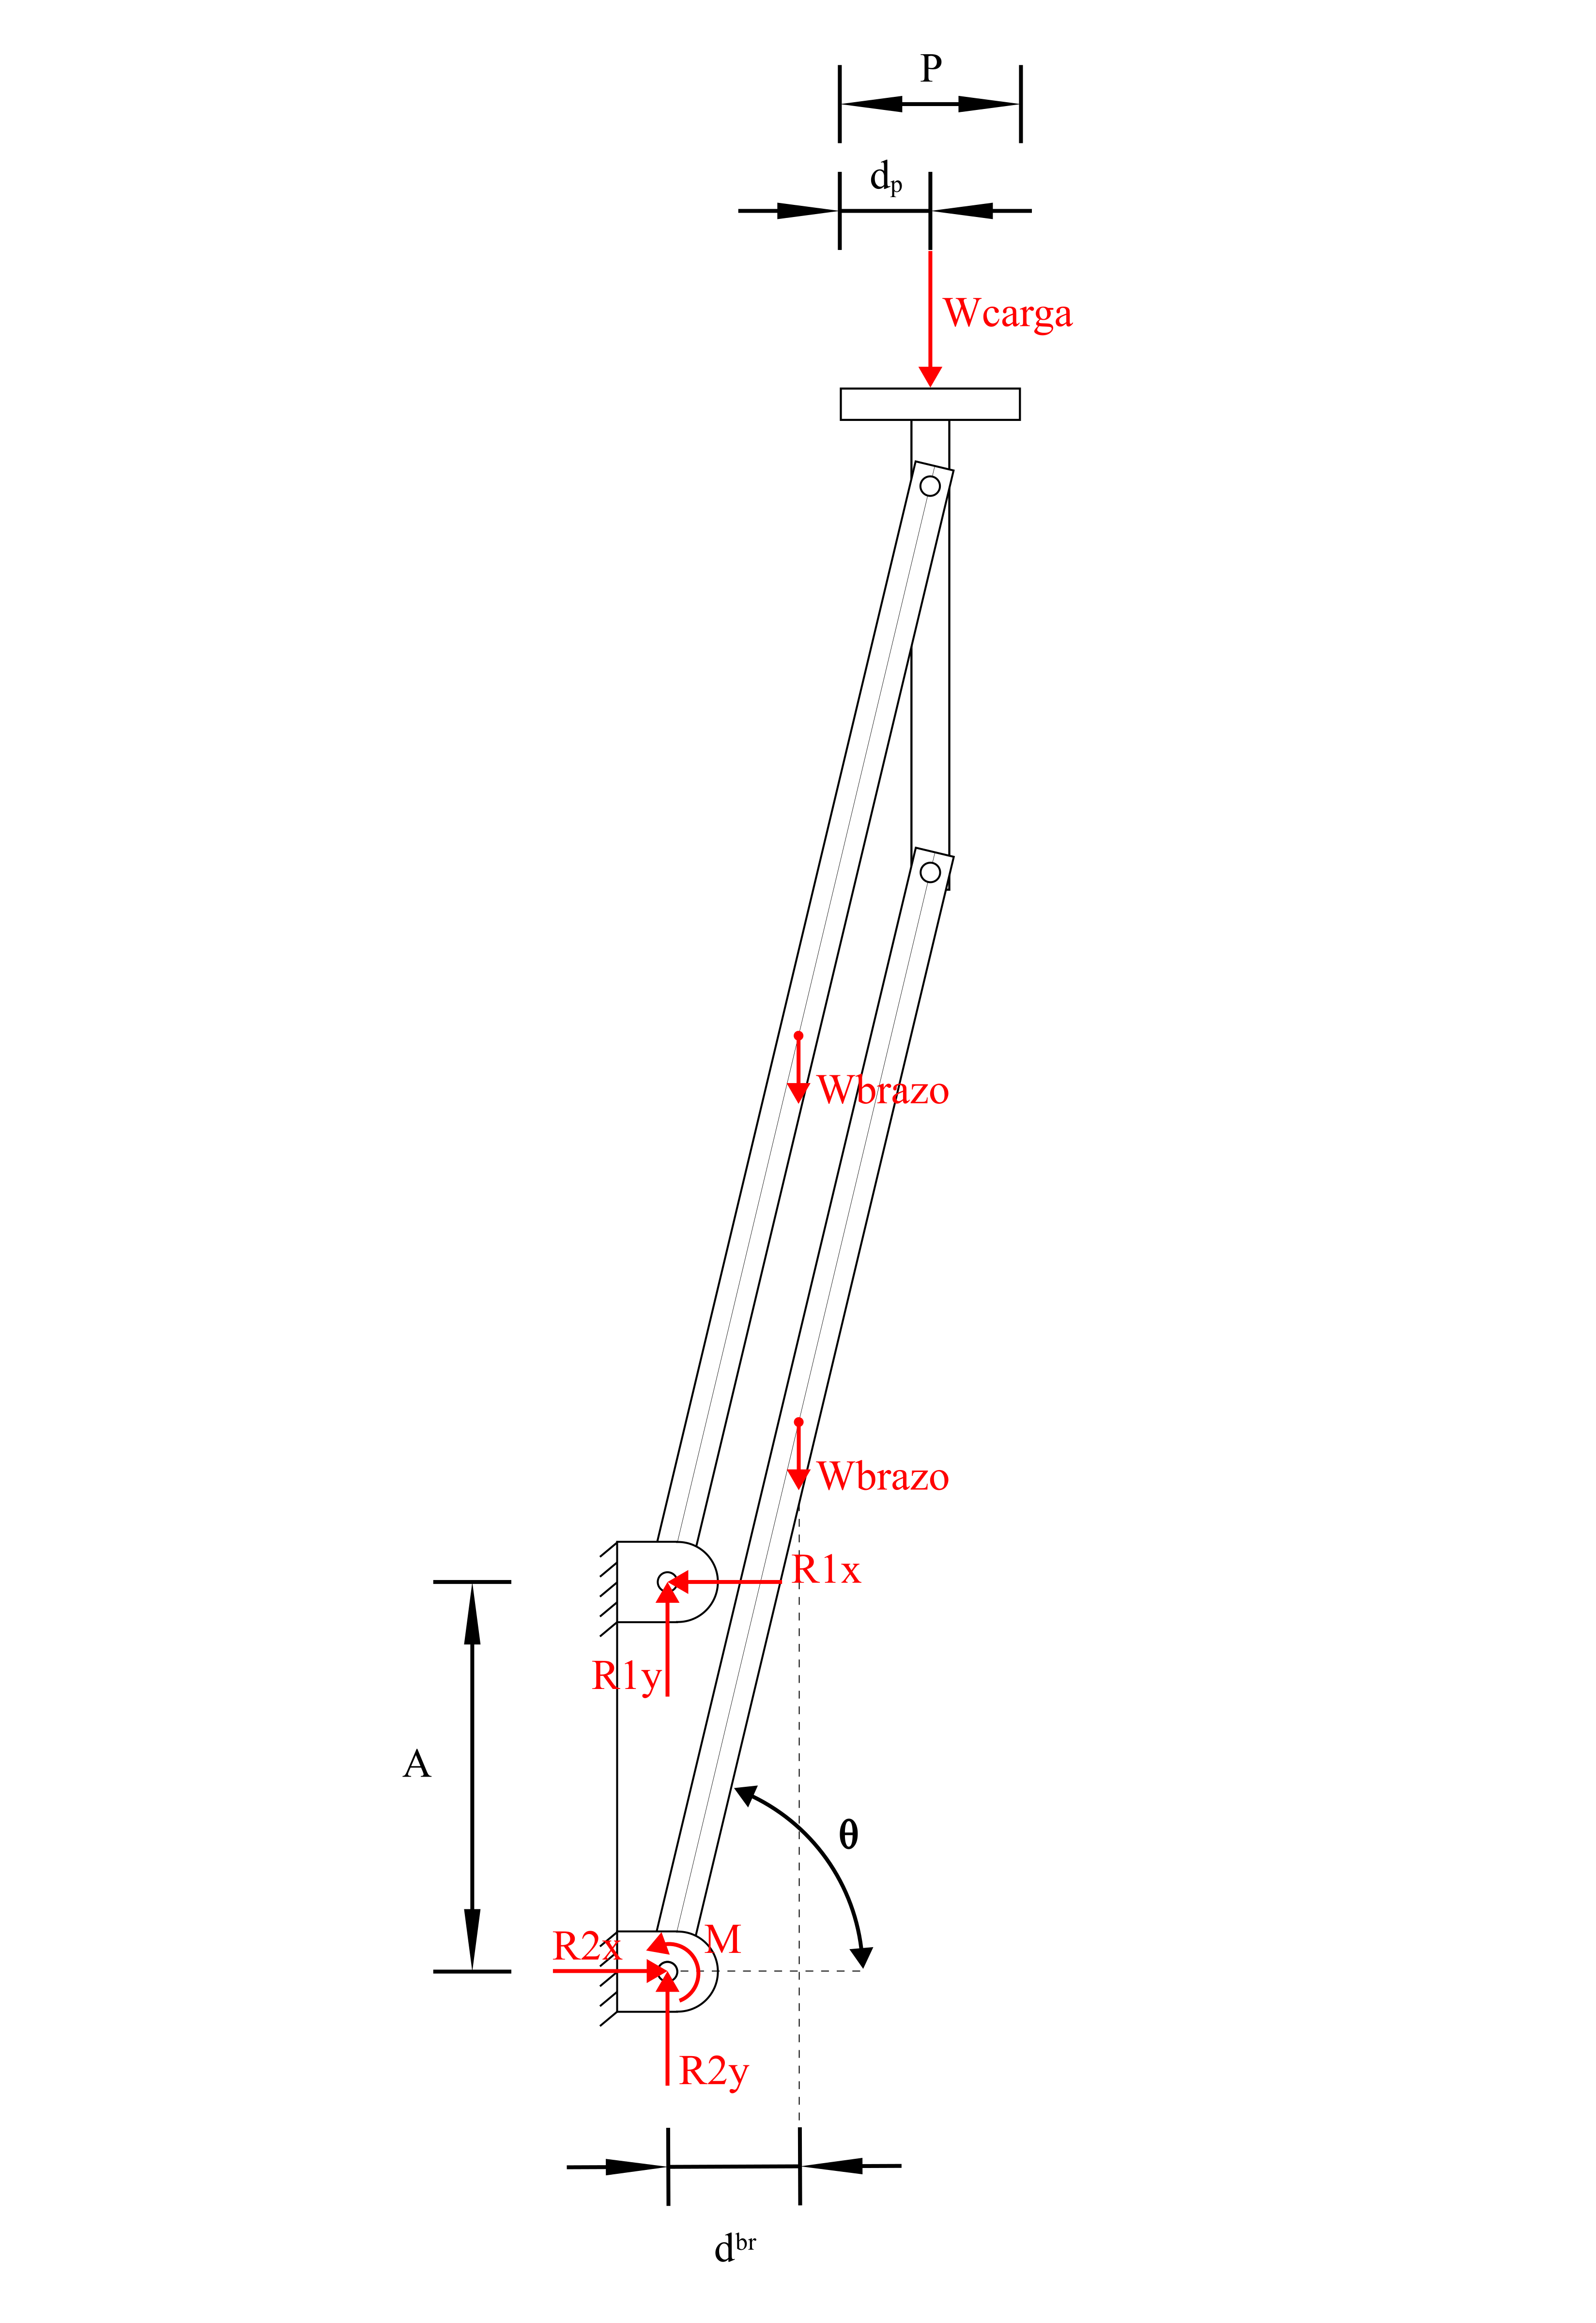
\includegraphics[width=\linewidth]{Recursos/Imagenes/ImagenesDisenoMecanico/4Bar_DCL_2.png}
	\end{minipage}
	\par\medskip

	\raggedright
	\footnotesize \textit{Nota.} Elaboración propia.
	\label{fig:DCLSubsistemaElevacion}
\end{figure}
% PENDIENTE: actualizar el esquema y el DCL con L, A, z_p, z_c, las cargas de viento, la pendiente y los resortes.

\subsubsection{Geometría y alcance}

En el paralelogramo, el acoplador describe un arco de radio $L$ sin rotar. La altura del plano óptico sobre el suelo en función del ángulo de los brazos es:

\begin{equation}\label{eq:altura_elev}
    H(\theta) = z_p + L \sin\theta + A + z_c
\end{equation}

Esta relación reproduce la altura medida en el modelo CAD con un error menor a $0.1\text{ mm}$. El ángulo máximo lo limita el contacto entre los brazos superior e inferior. La distancia perpendicular entre ellos es $A\cos\theta$, y en el modelo CAD entran en contacto en $\theta = 77^\circ$, cuando esta se reduce a $33.7\text{ mm}$. El ángulo máximo de operación se fija en:

\begin{equation}\label{eq:theta_max_elev}
    \theta_{\text{máx}} = \theta_{\text{choque}} - \Delta\theta_{h} = 77^\circ - 6.69^\circ = 70.31^\circ
\end{equation}

Con la Ecuación \ref{eq:altura_elev}, el plano óptico se ubica entre $904.0\text{ mm}$ ($\theta = 15^\circ$) y $1313.6\text{ mm}$ ($\theta = 70.31^\circ$), con un recorrido vertical de $409.6\text{ mm}$. En la posición baja, el subsistema de orientación sobresale $240.6\text{ mm}$ por delante de la cara frontal del chasis. En esa posición los brazos descansan sobre un soporte fijo a la base, de modo que no llegan a la horizontal.
% PENDIENTE: diseñar el soporte inferior (tope en theta = 15°).

La geometría del acoplador fija dos holguras adicionales. El tubo sobresale $25\text{ mm}$ más allá del pivote superior, y su esquina más alta sube a lo sumo $\sqrt{25^2 + 15.875^2} = 29.6\text{ mm}$ sobre el pivote, en $\theta = 57.6^\circ$. Como el pivote está a $43\text{ mm}$ de la cara superior del alma, la holgura mínima con la cara inferior del alma es de $10.4\text{ mm}$. En $\theta_{\text{máx}}$, la luz entre el brazo superior y el inferior es de $18.8\text{ mm}$, y la cartela superior con su tornillería ocupa $9.0\text{ mm}$, de modo que quedan $9.8\text{ mm}$ libres.

\subsubsection{Perfil de movimiento}

La plataforma recorre el barrido completo con un perfil trapezoidal de velocidad, igual al del subsistema de orientación: acelera durante $t_a = f_a\,t_b$, se mueve a velocidad constante y desacelera durante el mismo $t_a$. La velocidad angular máxima y la aceleración angular son:

\begin{equation}\label{eq:perfil_elev}
    \omega_{\text{máx}} = \frac{\Delta\theta}{t_b - t_a}, \qquad \ddot{\theta} = \frac{\omega_{\text{máx}}}{t_a}
\end{equation}

Para el barrido completo, $\Delta\theta = 55.31^\circ$ ($0.9653\text{ rad}$). Con $t_b = 10\text{ s}$ y $f_a = 0.25$, se obtiene $\omega_{\text{máx}} = 0.1287\text{ rad/s}$ ($7.37^\circ/\text{s}$, $1.23\text{ rpm}$) y $\ddot{\theta} = 0.0515\text{ rad/s}^2$. La velocidad máxima de cambio de altura es $L\cos\theta_{\text{mín}}\,\omega_{\text{máx}} = 74.6\text{ mm/s}$. El tiempo de barrido es un compromiso: un ajuste lento resta tiempo a la jornada del robot, pero los cambios de altura no son frecuentes y un movimiento suave evita excitar vibraciones en el sensor antes de medir.

Los ajustes en ruta usan la misma velocidad máxima y la misma aceleración, por lo que un movimiento más corto tarda menos. Un ajuste típico del plano óptico de $1000$ a $1300\text{ mm}$ ($\theta$ de $24.8^\circ$ a $66.8^\circ$) dura $8.2\text{ s}$.

\subsubsection{Cargas sobre el mecanismo}

El momento gravitacional en el pivote actuado se obtiene por trabajo virtual: como el acoplador se traslada sin rotar, este principio da el momento sin necesidad de resolver las fuerzas internas. Cada punto del acoplador desciende $L\cos\theta\,\delta\theta$ por cada giro $\delta\theta$ de los brazos, y el centro de masa de cada brazo desciende la mitad. Con el robot sobre una pendiente $\varphi$, el ángulo de los brazos respecto a la horizontal verdadera pasa a ser $\theta - \varphi$, y el momento total es:

\begin{equation}\label{eq:Mg_elev}
    M_g(\theta, \varphi) = \left(m_c + 2\,m_b\right) g\, L \cos(\theta - \varphi)
\end{equation}

donde $m_c = m_{\text{blk}} + m_U + m_h = 2.423\text{ kg}$ es la masa que se traslada con el acoplador. El factor $2\,m_b$ reúne los cuatro brazos, cada uno con su centro de masa a $L/2$ de su pivote. El momento no depende de la posición de la carga sobre el acoplador. Su valor máximo es $M_g = 18.65\text{ N}\cdot\text{m}$ y ocurre cuando $\theta = \varphi$, es decir, con los brazos paralelos a la horizontal verdadera en el extremo inferior del recorrido y el robot sobre una pendiente de la misma magnitud.

La carga de viento se calcula con la norma NTE E.020 \citep{nte_e020}, con el mismo criterio que en el subsistema de orientación:

\begin{equation}\label{eq:viento_elev}
    P = f_r \cdot 0.005\, C\, V^2 = 50.63\text{ kgf/m}^2 = 496.5\text{ Pa}
\end{equation}

La norma exige considerar el viento en dos direcciones horizontales perpendiculares. En dirección lateral, la presión actúa sobre el subsistema de orientación ($5.96\text{ N}$), sobre la cara de un ala del acoplador ($3.60\text{ N}$) y sobre la cara lateral completa de cada brazo, de $650\text{ mm}$ ($10.25\text{ N}$). Estas fuerzas no producen momento alrededor del eje de los pivotes, pero generan un momento de alabeo alrededor de la dirección de avance. Respecto al pivote inferior del acoplador, el momento es:

\begin{equation}\label{eq:Mr_elev}
    M_r = F_{\text{blk}}\, z_{\text{blk}} + F_{\text{ala}}\, z_{\text{ala}} + 2\,\frac{F_{\text{brazo}}}{2}\, A = 3.612\text{ N}\cdot\text{m}
\end{equation}

donde los brazos superiores entregan la mitad de su carga en el pivote superior. Este momento se equilibra con fuerzas verticales opuestas en los dos lados del mecanismo, separados $w_c = 173.4\text{ mm}$ entre los planos medios de los brazos:

\begin{equation}\label{eq:dV_elev}
    \Delta V = \pm\frac{M_r}{w_c} = \pm 20.8\text{ N}
\end{equation}

En la base, el momento de alabeo de todo el conjunto alcanza $22.12\text{ N}\cdot\text{m}$ en $\theta_{\text{máx}}$, con fuerzas verticales opuestas de $\pm 127.6\text{ N}$ en los pivotes de cada lado. Estas fuerzas cargan el marco inferior y los nodos de la base (Sección \ref{subsubsec:reacciones_elev}).

En dirección longitudinal, el viento actúa en el plano del mecanismo y sí produce momento en el pivote actuado. Las fuerzas son de $3.97\text{ N}$ sobre el área frontal del subsistema de orientación, de $0.63\text{ N}$ sobre los cantos de las alas del acoplador, y de $2.51$ a $7.85\text{ N}$ sobre cada brazo, cuya área frontal $b\,(L_t\sin\theta + h\cos\theta)$ crece con el ángulo. Por trabajo virtual, las fuerzas sobre el acoplador actúan con el brazo $L\sin\theta$ y las fuerzas sobre los brazos con $(L/2)\sin\theta$:

\begin{equation}\label{eq:Mv_elev}
    M_v(\theta) = \left(F_{\text{blk},x} + F_{U,x}\right) L\sin\theta + 4\,P\, b\left(L_t\sin\theta + h\cos\theta\right)\frac{L}{2}\sin\theta
\end{equation}

donde $b = 25.40\text{ mm}$ y $h = 31.75\text{ mm}$ son el ancho y el alto del tubo, y $L_t = 650\text{ mm}$ es su longitud de corte. A diferencia del momento gravitacional, $M_v$ crece con el ángulo: vale $1.49\text{ N}\cdot\text{m}$ en $\theta = 15^\circ$ y $11.47\text{ N}\cdot\text{m}$ en $\theta_{\text{máx}}$.

La fricción de las ocho chumaceras KFL08 se acota con el valor calculado para los rodamientos del eje basculante con el modelo de SKF \citep{skf2020bearings}, de $0.0201\text{ N}\cdot\text{m}$ por rodamiento. Ese valor corresponde a un rodamiento 6000-2RSH, cuyos sellos son mayores que los de un rodamiento 608, por lo que la cota es conservadora: $T_{\text{rod}} \leq 0.161\text{ N}\cdot\text{m}$.

\subsubsection{Reacciones en los nodos}\label{subsubsec:reacciones_elev}

Las fuerzas en los pasadores se obtienen con el equilibrio plano de los tres cuerpos del paralelogramo: los dos niveles de brazos y el acoplador. Los brazos superiores no llevan torque ni están unidos al travesaño, de modo que solo reciben las fuerzas de sus pasadores, su peso y el viento. Los brazos inferiores reciben además el torque del reductor y la fuerza de las patas móviles de los resortes sobre la varilla transversal, a $28\text{ mm}$ del pivote. Las incógnitas son las dos componentes de la fuerza en cada uno de los cuatro pivotes y el torque del reductor, nueve en total, y se resuelven con las tres ecuaciones de equilibrio de cada cuerpo. El peso actúa en la dirección de la gravedad con el robot sobre la pendiente $\varphi$, y el viento longitudinal en los dos sentidos. El torque que resulta del equilibrio coincide con el de la Ecuación \ref{eq:Tout_elev}, lo que verifica el modelo.

A cada reacción se le suma, del lado cargado, la fuerza vertical por el viento lateral ($\pm 20.8\text{ N}$ en el acoplador y $\pm 127.6\text{ N}$ en la base). La envolvente sobre todo el barrido, la pendiente y los dos sentidos del viento da, por lado, $70.0\text{ N}$ en el pivote inferior del acoplador y $59.1\text{ N}$ en el superior, y $240.1\text{ N}$ en el pivote inferior de la base y $166.2\text{ N}$ en el superior. Cada brazo superior trabaja como biela con una fuerza de hasta $41.5\text{ N}$. Como su línea de acción forma el ángulo $\theta$ con la horizontal, el momento que equilibra sobre el acoplador tiene un brazo de palanca $A\cos\theta$, que se reduce en las posiciones altas.

\subsubsection{Compensación con resortes de torsión}\label{subsubsec:resortes_elev}

El momento gravitacional es la mayor carga del mecanismo y actúa siempre en el mismo sentido. Para reducir el torque que debe entregar el motorreductor, se instalan dos resortes de torsión comerciales de Lee Spring, de acero inoxidable 302 y posición libre de $270^\circ$, uno por lado y coaxiales con el pivote actuado \citep{leespring_torsion}. Cada resorte se monta sobre un casquillo fijo, entre las chumaceras de los brazos inferiores. Una pata (la pata móvil) empuja hacia arriba una varilla transversal fija a los brazos inferiores, y la otra (la pata fija) reacciona contra una varilla de anclaje que une las dos placas de la base.

El catálogo da para este resorte, en alambre musical, un momento de $40\text{ lb}\cdot\text{in}$ a una deflexión de $270^\circ$, y un factor de $0.933$ para el acero inoxidable 302 \citep{leespring_torsion}. El momento nominal es entonces $M_{\text{nom}} = 40 \cdot 0.933 \cdot 0.112985 = 4.217\text{ N}\cdot\text{m}$ y la rigidez es $k = M_{\text{nom}}/\theta_{\text{nom}} = 0.895\text{ N}\cdot\text{m/rad}$. El momento de los dos resortes es:

\begin{equation}\label{eq:Ms_elev}
    M_s(\theta) = n_s\left[M_{\text{alto}} + k\left(\theta_{\text{máx}} - \theta\right)\right]
\end{equation}

con $n_s = 2$ y una precarga de $M_{\text{alto}} = 2.5\text{ N}\cdot\text{m}$ por resorte en la posición alta. Cada resorte trabaja entre $160^\circ$ (posición alta) y $215^\circ$ (posición baja) de deflexión, y el momento compensador total varía entre $5.00\text{ N}\cdot\text{m}$ ($\theta_{\text{máx}}$) y $6.73\text{ N}\cdot\text{m}$ ($\theta_{\text{mín}}$). La precarga se eligió moderada a propósito. Como la transmisión obliga al motor a impulsar la carga en ambos sentidos (Sección \ref{subsubsec:torque_elev}), una compensación excesiva solo invierte el signo del torque sin reducir su módulo. La posición libre de las patas tiene una tolerancia de $\pm 15^\circ$ para resortes de $11$ a $20$ espiras \citep{leespring_torsion}, que equivale a $\pm 0.234\text{ N}\cdot\text{m}$ por resorte; esta variación se incluye en la envolvente del torque de la Sección \ref{subsubsec:torque_elev}.

Los resortes de torsión se diseñan para cerrarse en servicio, y los esfuerzos residuales del enrollado solo favorecen al resorte si la carga se aplica en el sentido de las espiras \citep{Shigley11th}; el fabricante indica lo mismo \citep{leespring_torsion}. Por ello, la pata móvil sale tangente por la parte superior de la espira, paralela al brazo, y la pata fija sale hacia abajo y hacia adelante, tangente a $\psi = 230.4^\circ$ medido desde la horizontal delantera. Con las patas fijas hacia el exterior, junto a las chumaceras, el resorte del lado libre es de mano izquierda (LTL135T~03~S) y el del lado motor, de mano derecha (LTR135T~03~S). La pata móvil apoya en la varilla transversal a $28\text{ mm}$ del pivote, antes del ala de las cartelas, que empieza a $35\text{ mm}$. La pata fija apoya en la varilla de anclaje a $34\text{ mm}$ de su punto de tangencia. Las patas del catálogo ($A = 101.6\text{ mm}$) se cortan a $A \approx 39\text{ mm}$ (móvil) y $A \approx 45\text{ mm}$ (fija). La Tabla \ref{tab:resortes_elev} resume las fuerzas.

\begin{center}
    \footnotesize
    \begin{xltabular}{0.9\textwidth}{|X|>{\centering\arraybackslash}p{3cm}|>{\centering\arraybackslash}p{2.5cm}|}
        \caption{Fuerzas de los resortes en la posición baja, por resorte, incluida la tolerancia de posición libre\label{tab:resortes_elev}} \\
        \hline
        \rowcolor[HTML]{D9E1F2}
        Elemento & Brazo de palanca [mm] & Fuerza [N] \\ \hline
        \endfirsthead

        \multicolumn{3}{c}%
        {\tablename\ \thetable{} -- Continuación de la página anterior} \\
        \hline
        \rowcolor[HTML]{D9E1F2}
        Elemento & Brazo de palanca [mm] & Fuerza [N] \\ \hline
        \endhead

        \hline
        \endfoot

        \hline
        \endlastfoot

        Pata móvil sobre la varilla transversal & $28$ & $128.5$ \\ \hline
        Pata fija sobre la varilla de anclaje & $34$ & $105.8$ \\ \hline
        Resultante sobre el casquillo & -- & $146.1$ \\ \hline
    \end{xltabular}
\end{center}

La resistencia del resorte se verifica con el momento máximo del catálogo, que el fabricante define como la carga de diseño que evita la sobrecarga del resorte \citep{leespring_torsion}. El momento máximo de servicio, con la tolerancia de posición libre, es de $3.598\text{ N}\cdot\text{m} \leq 4.217\text{ N}\cdot\text{m}$. Como referencia, el esfuerzo de flexión según \citet{Shigley11th}, con el factor de corrección por curvatura $K_i = 1.094$ para el índice $C = 8.64$, es de $929\text{ MPa}$ en la posición baja. Para el alambre de acero inoxidable 302, el mismo texto estima $S_{ut} = 2065/d^{0.263} = 1493\text{ MPa}$ y $S_y = 0.61\,S_{ut} = 911\text{ MPa}$, y advierte que un resorte cargado en el sentido de las espiras puede trabajar por encima de la fluencia del alambre. El momento admitido por el fabricante corresponde a $1165\text{ MPa}$.

Al enrollarse, el diámetro de la espira se reduce \citep{Shigley11th}, por lo que se verifica la holgura con el casquillo. Si toda la deflexión se asigna al cuerpo y se suma la tolerancia de $+15^\circ$ (en total $230^\circ$), el diámetro interior baja a $24.96\text{ mm}$. Queda una holgura diametral de $2.96\text{ mm}$ con el casquillo de $\varnothing 22\text{ mm}$, más pequeño que el mandril sugerido de $23.81\text{ mm}$.

Las dimensiones del resorte condicionan el diseño del nodo inferior. Su diámetro exterior es de $33.05\text{ mm}$ y el cuerpo mide $54.0\text{ mm}$. Como suposición geométrica sin fuente, se considera que el cuerpo se alarga un diámetro de alambre ($3.43\text{ mm}$) por cada vuelta de deflexión, hasta $56.0\text{ mm}$ en la posición baja. Con una holgura de $3\text{ mm}$ entre resortes y chumaceras, el espacio entre las chumaceras de los dos brazos es de $121.1\text{ mm}$, que fija el ancho del mecanismo (Sección \ref{subsubsec:acoplador_elev}).

\subsubsection{Inercia y torque requerido}\label{subsubsec:torque_elev}

La inercia respecto al pivote actuado incluye la masa que se traslada con el acoplador, a la distancia $L$, y los cuatro brazos, que giran alrededor de sus pivotes base \citep{norton2020maquinaria}:

\begin{equation}\label{eq:J_elev}
    J = m_c L^2 + 4\, m_b\left(\frac{L_t^2}{12} + \frac{L^2}{4}\right) = 0.8722 + 0.1869 = 1.0591\text{ kg}\cdot\text{m}^2
\end{equation}

El reductor de tornillo sin fin no puede ser accionado desde la salida en reposo, por lo que el motor siempre debe impulsar la carga, incluso cuando la gravedad o el viento actúan a favor del giro. Por ello, el torque en el eje de salida se calcula sumando los módulos de todos los términos, y se toma la pendiente más desfavorable en cada ángulo:

\begin{equation}\label{eq:Tout_elev}
    T_{\text{out}}(t) = \max_{\varphi}\left|M_g\!\left(\theta(t), \varphi\right) - M_s\!\left(\theta(t)\right)\right| + \left|M_v\!\left(\theta(t)\right)\right| + T_{\text{rod}} + J\left|\ddot{\theta}(t)\right|
\end{equation}

El término inercial es de apenas $J\ddot{\theta} = 0.0545\text{ N}\cdot\text{m}$, por lo que el torque está dominado por las cargas estáticas. Con los resortes, el torque máximo en el eje de salida es de $18.75\text{ N}\cdot\text{m}$, en $\theta = 56.7^\circ$; sin ellos sería de $23.77\text{ N}\cdot\text{m}$, de modo que la compensación reduce el torque de diseño en un $21\%$. Su variación a lo largo del barrido se analiza en la Sección \ref{subsubsec:torque_tray_elev}. Este torque se reparte entre los dos brazos inferiores a través del marco rígido que forman el travesaño y las cartelas; el motorreductor entrega el total al brazo accionado.

\subsection{Dimensionamiento de componentes}\label{subsec:dimensionamiento_elev}

\subsubsection{Criterios de verificación}

Los componentes de aluminio se verifican con la especificación del \textit{Aluminum Design Manual} \citep{aluminum2005manual}, con sus factores de seguridad para estructuras tipo edificación: $n_u = 1.95$ respecto a la resistencia última, $n_y = 1.65$ respecto a la fluencia y $n_a = 1.20$ para la apariencia. Como ninguna pieza lleva soldadura, el coeficiente de tracción es $k_t = 1.0$. Las propiedades mínimas del 5052-H32 y del 6061-T6 se toman del mismo manual.

Los elementos de acero se verifican con los criterios de \citet{Shigley11th}: el esfuerzo de fluencia en corte se toma como $S_{sy} = 0.577\,S_y$ (teoría de la energía de distorsión), los ejes se verifican a fatiga con el criterio de Goodman modificado y a fluencia con el esfuerzo de Von Mises máximo, y se exige un factor de seguridad de al menos $1.5$. Las propiedades de los aceros AISI 4140, SAE 1045 y AISI 303 se toman de las fichas técnicas de los proveedores \citep{europer_4140, europer_1045, ficha_aisi303}. En el caso del AISI 4140 bonificado, la ficha aclara que las propiedades mecánicas son informativas y que solo la dureza está garantizada. La tornillería es de acero inoxidable A2-70, con $R_m = 700\text{ MPa}$ y $R_{p0.2} = 450\text{ MPa}$ \citep{iso3506_1_2020}; su resistencia al corte se toma como $0.577\,R_{p0.2}/n_y$ sobre el área resistente.

\subsubsection{Acoplador en U}\label{subsubsec:acoplador_elev}

El acoplador es una sola pieza de chapa de aluminio 5052-H32 de $3\text{ mm}$, cortada por láser y doblada en prensa plegadora en forma de U invertida (Figura \ref{fig:AcopladorU}). El alma, de $212 \times 34\text{ mm}$ interiores, sostiene la viga 2040 del subsistema de orientación, y las dos alas, de $34\text{ mm}$ de ancho y $213\text{ mm}$ de largo desde la cara superior del alma, alojan los pasadores de los pivotes superiores. El pivote superior está a $43\text{ mm}$ de la cara superior del alma, el inferior a $A = 150\text{ mm}$ por debajo de él, y bajo el pivote inferior quedan $20\text{ mm}$ de material. La masa de la pieza es de $0.174\text{ kg}$.

\begin{figure}[H]
	\captionsetup{justification=raggedright, singlelinecheck=false, labelsep=none}
	\caption[Acoplador en U del subsistema de elevación.]{}
	\textit{Acoplador en U del subsistema de elevación.} \par\medskip

	\centering
	% PENDIENTE: generar la figura del acoplador (plano o vista del CAD).
	
\includegraphics[width=0.7\linewidth]{Recursos/Imagenes/Placeholder.png}
	\par\medskip

	\raggedright
	\footnotesize \textit{Nota.} Elaboración propia.
	\label{fig:AcopladorU}
\end{figure}

El ancho $w$ entre las caras interiores de las alas es igual a la separación entre los brazos de la base, porque los dos pares de brazos son paralelos. Tres condiciones lo limitan: el apoyo de la viga 2040 sobre el alma exige al menos $66.6\text{ mm}$; la distancia entre los agujeros de la viga y el inicio del doblez, al menos $64.1\text{ mm}$; y el apilamiento de piezas en el nodo inferior, al menos:

\begin{equation}\label{eq:w_elev}
    w \geq 2\left(t_{\text{ar}} + t_{\text{tu}} + b + t_{\text{KFL}}\right) + g = 2\left(1.6 + 5 + 25.4 + 13\right) + 121.1 = 211.1\text{ mm}
\end{equation}

donde $t_{\text{ar}}$ es el espesor de la arandela DIN 125 A 8.4, $t_{\text{tu}}$ el de la tuerca, $b$ el ancho del tubo, $t_{\text{KFL}}$ el alto de la chumacera y $g$ el espacio que ocupan los resortes (Sección \ref{subsubsec:resortes_elev}). Como gobierna el apilamiento, se adopta $w = 212\text{ mm}$. La distancia entre los planos medios de los brazos de cada lado es entonces $w_c = 173.4\text{ mm}$, y el travesaño del marco inferior mide $147\text{ mm}$.

El radio interior de doblado mínimo para el 5052-H32 de $3\text{ mm}$ es de $3.0\text{ mm}$ \citep{astm_b209m}. Las tolerancias generales siguen la clase media de la norma ISO 2768-1 \citep{iso2768_1}, que da $\pm 1^\circ$ para el ángulo de cada doblez. Para que los dos pivotes de cada ala queden alineados con los de la otra, los agujeros de $\varnothing 8\text{ H7}$ se escarian después del doblado, en una sola sujeción y referidos al alma. Los cuatro agujeros de $\varnothing 5.5\text{ mm}$ para la viga 2040 (serie media de ISO 273 \citep{iso273} para M5) se desplazan $10.3\text{ mm}$ respecto al plano medio, de modo que el centro de masa del subsistema de orientación, desplazado hacia el motor NEMA 17, quede sobre el plano medio del mecanismo.

La flexión del alma bajo la carga de la viga gobierna el diseño del acoplador: el esfuerzo es de $25.6\text{ MPa}$ frente a un admisible de $97.0\text{ MPa}$, con un factor de seguridad de $3.8$. Las distancias al borde de los agujeros de los pasadores ($17.0$ y $20.0\text{ mm}$) y de los tornillos de la viga ($10.75\text{ mm}$) superan $2D$, de modo que la capacidad de aplastamiento no se reduce, y la separación entre tornillos cumple el mínimo de $2.5D$ \citep{aluminum2005manual}. El aplastamiento del pasador en el ala se calcula con la mayor reacción de los nodos del acoplador ($70.0\text{ N}$) y con el área nominal $D\,t$, aunque el agujero apoya sobre la rosca del pasador (Sección \ref{subsubsec:nodos_elev}). Esta verificación y la extracción de las tuercas en T de la viga tienen factores mucho mayores (Tabla \ref{tab:resumen_fs_elev}).

\subsubsection{Pasadores y chumaceras de los nodos}\label{subsubsec:nodos_elev}

Cada nodo del acoplador lleva un solo pasador de $\varnothing 8 \times 242\text{ mm}$ de acero AISI 4140 bonificado, que atraviesa las dos alas (Figura \ref{fig:PasadorElev}). Su largo es la distancia de $218\text{ mm}$ entre las caras exteriores de las alas más $12\text{ mm}$ de rosca para cada perilla. Cada extremo tiene $20\text{ mm}$ de rosca M8, que alojan la perilla, el ala y la tuerca; los $202\text{ mm}$ centrales están rectificados a $\varnothing 8\text{ h6}$. Desde cada ala hacia el centro, el apilamiento es: tuerca, arandela DIN 125 A 8.4, tubo del brazo y chumacera KFL08. La perilla y la tuerca aprietan el ala entre ambas, de modo que el pasador queda fijo al acoplador y cada brazo gira sobre él a través de su chumacera. Los prisioneros del anillo interior de cada KFL08 se aprietan sobre un plano fresado en el pasador.

\begin{figure}[H]
	\captionsetup{justification=raggedright, singlelinecheck=false, labelsep=none}
	\caption[Pasador de un nodo del acoplador.]{}
	\textit{Pasador de un nodo del acoplador y piezas montadas sobre él.} \par\medskip

	\centering
	% PENDIENTE: generar la figura del pasador (vista longitudinal con rosca, zona rectificada y planos).
	
\includegraphics[width=0.85\linewidth]{Recursos/Imagenes/Placeholder.png}
	\par\medskip

	\raggedright
	\footnotesize \textit{Nota.} Elaboración propia.
	\label{fig:PasadorElev}
\end{figure}

Como la tuerca se monta desde el extremo del pasador, la rosca pasa también por el agujero del ala, y el agujero de $\varnothing 8\text{ H7}$ apoya sobre las crestas de la rosca y no sobre la zona rectificada. Se aceptó esta solución por su simplicidad, con dos consecuencias. La primera es que el juego entre las crestas de la rosca y el agujero anula el ajuste H7; la posición del pasador la fija en la práctica el apriete entre la perilla y la tuerca. La segunda es que la flexión del pasador junto al ala se verifica en la sección roscada, con el diámetro equivalente al área resistente, $d_s = d - 0.9382\,p = 6.83\text{ mm}$ \citep{iso3506_1_2020}.

Con un brazo de palanca de $38.5\text{ mm}$ entre la cara interior del ala y el plano medio de la chumacera, el esfuerzo en la rosca es de $86.3\text{ MPa}$ en los nodos del acoplador ($70.0\text{ N}$) y de $204.8\text{ MPa}$ en el lado libre del pivote superior de la base ($166.2\text{ N}$). El límite de fluencia del 4140 es de $900\text{ MPa}$ para diámetros de hasta $16\text{ mm}$ \citep{europer_4140}, de modo que ambos esfuerzos quedan por debajo del admisible $S_y/n_y = 545.5\text{ MPa}$, con factores de seguridad de $10.4$ y $4.4$ respecto a la fluencia. En el lado accionado del pivote superior, el separador lleva el brazo de palanca a $57.9\text{ mm}$, pero la sección junto a la placa es de $\varnothing 8\text{ mm}$ llena: el esfuerzo es de $191.4\text{ MPa}$, con un factor de seguridad de $4.7$. El pasador del pivote actuado, que se verifica en la Sección \ref{subsubsec:pasador_base_elev}, exige el 4140, y se usa el mismo material en todos los pasadores.

Las chumaceras KFL08 llevan un rodamiento con capacidad estática $C_0 = 1.6\text{ kN}$ y dinámica $C = 4.2\text{ kN}$ \citep{madler_kfl08}. Con la mayor reacción radial, de $240.1\text{ N}$ en la base, el factor de seguridad estático es $S_0 = C_0/P_0 = 6.7$. Como el mecanismo gira a menos de $1.3\text{ rpm}$ y solo durante los ajustes, la vida a fatiga del rodamiento no es una limitación. Cada chumacera se fija a la pared interior del tubo con dos tornillos M4 A2-70 y tuercas dentro del tubo, en los agujeros de $\varnothing 5\text{ mm}$ de la pieza; el agujero exterior queda a $6.75\text{ mm} = 1.69D$ del extremo del tubo, y los tornillos y la pared trabajan con factores amplios (Tabla \ref{tab:resumen_fs_elev}). La carcasa de aleación de zinc no tiene una capacidad publicada; las cargas son bajas, pero esta es una limitación del análisis.

\subsubsection{Pasadores de la base}\label{subsubsec:pasador_base_elev}

En el lado accionado, el pasador del pivote actuado no puede cruzar al exterior del brazo, donde se ubica el reductor. Por ello, este pasador es un voladizo de $\varnothing 8\text{ h6} \times 196.5\text{ mm}$ de AISI 4140 ($22\text{ mm}$ de rosca M8 y $174.5\text{ mm}$ rectificados), fijo en la placa del lado libre con la perilla y la tuerca. Atraviesa el brazo libre y su chumacera y el casquillo de los resortes, y termina dentro de la chumacera del brazo accionado, $0.5\text{ mm}$ antes de la cara del tubo. Bajo los cubos de las dos chumaceras lleva planos fresados de $0.5\text{ mm}$ para los prisioneros. El casquillo de los resortes es de POM-C, de $\varnothing 22 \times \varnothing 8.1 \times 120.5\text{ mm}$, elegido entre seis plásticos por su temperatura de servicio, su baja absorción de humedad y su resistencia.

El pasador recibe la reacción del brazo libre ($240.1\text{ N}$ a $38.5\text{ mm}$ del apoyo) y la resultante de cada resorte sobre el casquillo ($146.1\text{ N}$, con la tolerancia de posición libre). Como voladizo puro, la sección roscada junto al apoyo llegaría a $1287.5\text{ MPa}$, por lo que el pasador depende de que la chumacera del brazo accionado guíe su extremo. Si el eje del reductor está alineado con el pasador sin carga, la guía toma $151.8\text{ N}$ y la sección roscada trabaja a $444.3\text{ MPa}$, con un factor de seguridad de $2.03$ respecto a la fluencia. La desalineación admisible del eje del reductor en el sentido más desfavorable es de $0.76\text{ mm}$. Con la tolerancia de coaxialidad especificada de $0.7\text{ mm}$, el esfuerzo es de $537.3\text{ MPa}$ y el factor de seguridad, de $1.68$. Recorriendo todo el pasador con la desalineación en los dos sentidos, la sección más esforzada sigue siendo la roscada junto al apoyo; los planos fresados trabajan a menos. La chumacera del brazo libre tiene $S_0 = 6.7$.

El pasador del pivote superior de la base es de $\varnothing 8 \times 267.9\text{ mm}$ de AISI 4140 y se fija en las dos placas con perillas. En el lado libre lleva el mismo apilamiento que el pivote actuado (perilla, placa, tuerca y arandela). En el lado accionado, un separador de $\varnothing 14 \times \varnothing 8.2 \times 25.8\text{ mm}$ ubica el brazo respecto a la placa con $0.2\text{ mm}$ de juego, para que el apriete de la perilla no cargue la chumacera en dirección axial ni frene el giro del brazo. La rosca de ese extremo entra $1\text{ mm}$ en la placa para que la perilla apriete.

\subsubsection{Marco inferior: travesaño y cartelas}

El travesaño es un tramo de $147\text{ mm}$ del mismo tubo de los brazos, ubicado a $65\text{ mm}$ del pivote de la base. Se une a los brazos solo mediante cuatro cartelas en T de 5052-H32 de $3\text{ mm}$, dos por encima y dos por debajo, con tornillos pasantes M5 A2-70. Cada tornillo atraviesa el tubo por dentro de un separador de acero inoxidable 303 de $\varnothing 8 \times \varnothing 5.4\text{ mm}$ y $27.75\text{ mm}$ de largo, que evita aplastar el tubo al apretar, y lleva arandelas DIN 125 A 5.3 y tuerca autoblocante DIN 985. El ala de cada cartela ($60 \times 25.4\text{ mm}$) se fija al brazo con dos tornillos sobre su eje, a $45$ y $85\text{ mm}$ del pivote; el tallo ($32.5 \times 20\text{ mm}$) se fija al travesaño con dos tornillos separados $12.5\text{ mm}$.

La carga de diseño del marco es la torsión del travesaño, que transmite al brazo no accionado la mitad del torque de gravedad y viento y resiste además el momento de alabeo del viento lateral. La torsión de diseño es $T_t = 19.13\text{ N}\cdot\text{m}$, en $\theta = 22.5^\circ$ y con la pendiente de $16^\circ$, incluida la tolerancia de posición libre de los resortes. Las cartelas superior e inferior forman un par de fuerzas con brazo $h = 34.75\text{ mm}$, de modo que cada cartela recibe $F = 550.6\text{ N}$.

El momento en el plano de cada cartela se reparte entre los dos grupos de tornillos según su rigidez rotacional, proporcional a $\sum r^2$ \citep{Shigley11th}: el grupo del brazo toma el $91\%$ y el del travesaño el $9\%$. El tornillo más cargado recibe $396.0\text{ N}$, frente a una capacidad al corte de $2232\text{ N}$, con un factor de seguridad de $5.64$; el aplastamiento en la cartela y en la pared del tubo tiene factores mayores. Las distancias al borde de las cartelas y las separaciones cumplen los mínimos de $2D$ y $2.5D$. En el travesaño, el tornillo queda a $9.5\text{ mm}$ del extremo del tubo ($1.9D$), por encima del mínimo de $1.5D$, con una reducción del $5\%$ en la capacidad de aplastamiento de la pared \citep{aluminum2005manual}.

La cartela y el travesaño trabajan con esfuerzos bajos. En el cuello de la T, la flexión da $12.5\text{ MPa}$ frente a $114.1\text{ MPa}$ admisibles por pandeo local. La torsión del travesaño, como tubo cerrado de pared delgada, da $\tau = T_t/(2A_m t) = 6.9\text{ MPa}$ frente a $84.0\text{ MPa}$ admisibles.

La precarga de los tornillos se limita a $F_i = 0.55\,A_s R_{p0.2} = 3.51\text{ kN}$, porque el separador de AISI 303 no admite más: con esa precarga trabaja a $128.3\text{ MPa}$, por debajo de su admisible de $136.4\text{ MPa}$. El par de apriete es $T = K F_i d = 3.51\text{ N}\cdot\text{m}$, con $K = 0.20$ \citep{Shigley11th}, al que se suma el par de rozamiento propio de la tuerca DIN 985. La unión no cuenta con la fricción entre placas, por lo que los tornillos se verifican al corte y al aplastamiento.

\subsubsection{Brazos}

Los cuatro brazos son tubos rectangulares de 6061-T6 de $31.75 \times 25.4 \times 2\text{ mm}$ y $600\text{ mm}$ entre pivotes ($A = 212.6\text{ mm}^2$, $I_x = 29\,638\text{ mm}^4$ en el plano del mecanismo, $I_y = 20\,694\text{ mm}^4$, $S_x = 1867\text{ mm}^3$). Se verifican a carga axial combinada con flexión \citep{aluminum2005manual}, con los esfuerzos admisibles de la Tabla \ref{tab:brazos_adm_elev} y la envolvente de ángulos, pendientes y viento de la Sección \ref{subsubsec:reacciones_elev}. Cada brazo recibe la mitad de las fuerzas de los pasadores de su nivel, su peso y el viento repartidos a lo largo, y, en los brazos inferiores, la mitad de la fuerza de las patas móviles a $28\text{ mm}$ del pivote. El brazo accionado recibe el torque completo del reductor y entrega la mitad al otro brazo inferior por el travesaño. Se toma $k = 1$ en los dos planos, $C_m = 1$ y, de forma conservadora, los anchos planos de las paredes iguales al lado exterior menos dos espesores.

\begin{center}
    \footnotesize
    \begin{xltabular}{0.9\textwidth}{|X|>{\centering\arraybackslash}p{4.5cm}|>{\centering\arraybackslash}p{2.8cm}|}
        \caption{Esfuerzos admisibles de los brazos de 6061-T6 según el \textit{Aluminum Design Manual}\label{tab:brazos_adm_elev}} \\
        \hline
        \rowcolor[HTML]{D9E1F2}
        Modo & Esbeltez & Admisible [MPa] \\ \hline
        \endfirsthead

        \multicolumn{3}{c}%
        {\tablename\ \thetable{} -- Continuación de la página anterior} \\
        \hline
        \rowcolor[HTML]{D9E1F2}
        Modo & Esbeltez & Admisible [MPa] \\ \hline
        \endhead

        \hline
        \endfoot

        \hline
        \endlastfoot

        Columna & $kL/r = 60.8$ & $86.0$ \\ \hline
        Paredes de columna & $b/t = 13.88$ & $134.9$ \\ \hline
        Ala comprimida & $b/t = 10.70$ & $145.5$ \\ \hline
        Alma en flexión & $h/t = 13.88$ & $189.1$ \\ \hline
        Pandeo lateral & $L_bS_c/(C_b\sqrt{I_yJ/2}) = 57.7$ & $145.5$ \\ \hline
        Tracción & -- & $145.5$ \\ \hline
    \end{xltabular}
\end{center}

El brazo más cargado es el inferior accionado, con un momento máximo de $20.42\text{ N}\cdot\text{m}$ junto a su pivote y una compresión de $47.5\text{ N}$; su índice de interacción es de $0.077$. El brazo inferior libre llega a $0.039$ y los superiores, que solo reciben las fuerzas de sus pasadores, su peso y el viento, a $0.004$. Ante el torque máximo permisible del reductor ($38\text{ N}\cdot\text{m}$), la raíz del brazo accionado trabaja a $20.4\text{ MPa}$. Los brazos están sobredimensionados para la resistencia, porque su sección la fijan la rigidez y el espacio para las chumaceras KFL08.

\subsubsection{Unión entre el reductor y el brazo accionado}\label{subsubsec:eje_salida_elev}

El reductor tiene un eje de salida hueco de $\varnothing 18\text{ mm}$ y $78\text{ mm}$ de largo, con chavetero de $6\text{ mm}$ \citep{stepperonline_nmrvs40}. La brida comercial que se atornilla al brazo tiene un agujero de $\varnothing 14\text{ mm}$; una brida para $\varnothing 18\text{ mm}$ tendría su círculo de tornillos fuera de la cara de $31.75\text{ mm}$ del tubo. Por ello, la unión se resuelve con un eje escalonado de AISI 4140 bonificado (Figura \ref{fig:EjeSalida}), formado por:
\begin{itemize}
    \item un tramo de $\varnothing 18\text{ h6} \times 81\text{ mm}$ dentro del eje hueco, con chaveta DIN 6885-1 A $6 \times 6 \times 40$, retenido en el extremo opuesto con un anillo DIN 471 de $18\text{ mm}$;
    \item un collarín de $\varnothing 22 \times 2\text{ mm}$ que se apoya en el extremo del eje hueco, de $\varnothing 31\text{ mm}$;
    \item un tramo de $\varnothing 14\text{ h6} \times 25\text{ mm}$ dentro de la brida, con chaveta A $5 \times 5 \times 20$.
\end{itemize}

La brida es de acero AISI 303, con cubo de $\varnothing 24\text{ mm}$, $25\text{ mm}$ de largo total, ala de $\varnothing 36 \times 3\text{ mm}$ y cuatro agujeros de $\varnothing 3\text{ mm}$ en un círculo de $\varnothing 30\text{ mm}$. Se fija a la cara exterior del brazo con cuatro tornillos M3 A2-70, girados $45^\circ$ respecto al eje del tubo para que quepan en la cara, y con tuercas en la cara interior de la pared, a las que se accede por el extremo abierto del tubo.

\begin{figure}[H]
	\captionsetup{justification=raggedright, singlelinecheck=false, labelsep=none}
	\caption[Eje escalonado de salida del reductor.]{}
	\textit{Eje escalonado de salida del reductor y su unión con la brida y el brazo.} \par\medskip

	\centering
	% PENDIENTE: generar la figura del eje escalonado (corte del ensamble).
	
\includegraphics[width=0.85\linewidth]{Recursos/Imagenes/Placeholder.png}
	\par\medskip

	\raggedright
	\footnotesize \textit{Nota.} Elaboración propia.
	\label{fig:EjeSalida}
\end{figure}

Para la unión se consideran dos casos de torsión: la operación, con $T_{\text{op}} = S\,T_{\text{out}} = 24.37\text{ N}\cdot\text{m}$, y una sobrecarga igual al torque máximo permisible del reductor, $T_{\text{red}} = 38\text{ N}\cdot\text{m}$, de modo que la unión no sea más débil que el reductor. Como carga radial se toma, de forma conservadora, toda la reacción del pivote inferior de la base ($240.1\text{ N}$, Sección \ref{subsubsec:reacciones_elev}) aplicada en el plano medio del ala de la brida. Su brazo de palanca es de $24.5\text{ mm}$ hasta el hombro del tramo de $\varnothing 14\text{ mm}$ y de $29.0\text{ mm}$ hasta la cara de la carcasa.

Los factores de concentración de esfuerzos del eje son los valores estimados que da \citet{Shigley11th} para el primer dimensionamiento de un eje. Se combinan en la misma sección el peor valor de flexión (filete agudo, $K_t = 2.7$) y el peor de torsión (cuñero fresado, $K_{ts} = 3.0$), con sensibilidad a la muesca $q = 1$. El radio de filete adoptado, $r = 0.5\text{ mm}$, da $r/d = 0.036$, mayor que el $0.02$ que suponen esos valores, por lo que los factores son conservadores. La flexión se toma como completamente invertida y la torsión como repetida entre cero y su máximo. El límite de resistencia a la fatiga se corrige por superficie maquinada y por tamaño \citep{Shigley11th}:

\begin{equation}\label{eq:Se_eje_elev}
    S_e = k_a\,k_b\,(0.5\,S_{ut}), \qquad k_a = 3.04\,S_{ut}^{-0.217}, \qquad k_b = 1.24\,d^{-0.107}
\end{equation}

Con $S_y = 750\text{ MPa}$ y $S_{ut} = 1000\text{ MPa}$ para barras de $16$ a $40\text{ mm}$ \citep{europer_4140}, la sección de $\varnothing 14\text{ mm}$ tiene $S_e = 317\text{ MPa}$. El factor de seguridad a fatiga se obtiene con el criterio ED-Goodman \citep{Shigley11th}:

\begin{equation}\label{eq:goodman_elev}
    \frac{1}{n} = \frac{16}{\pi d^3}\left[\frac{\sqrt{4\left(K_f M_a\right)^2 + 3\left(K_{fs} T_a\right)^2}}{S_e} + \frac{\sqrt{4\left(K_f M_m\right)^2 + 3\left(K_{fs} T_m\right)^2}}{S_{ut}}\right]
\end{equation}

y el de fluencia, con el esfuerzo de Von Mises máximo. La sección crítica es la de $\varnothing 14\text{ mm}$, con un factor de seguridad de $1.88$ a fatiga en operación y de $2.02$ a fluencia con el torque de $38\text{ N}\cdot\text{m}$. En la sección de $\varnothing 18\text{ mm}$ los factores son mayores que $3.8$. El mismo eje en SAE 1045 tendría un factor de $0.92$ a fluencia en la sobrecarga, por lo que se adopta el 4140.

Las chavetas se verifican al corte sobre el área $b\,l_{\text{ef}}$ y al aplastamiento sobre la altura de contacto con el cubo \citep{Shigley11th}, con la longitud efectiva $l_{\text{ef}} = l - b$ por sus extremos redondeados. El chavetero de $6\text{ mm}$ del eje hueco tiene una profundidad de $2.8\text{ mm}$ en el cubo, medida en el modelo CAD y coincidente con la norma DIN 6885-1 \citep{din6885_1}; el del eje se mecaniza con la profundidad normalizada de $3.5\text{ mm}$. En cambio, el chavetero de la brida tiene $3.0\text{ mm}$ de profundidad en el cubo, más que los $2.3\text{ mm}$ de la norma. Con la profundidad normalizada en el eje ($3.0\text{ mm}$), la chaveta apoyaría solo $2.0\text{ mm}$ en el cubo de acero 303, que no alcanzaría el factor de $1.5$ en la sobrecarga. Por ello, el chavetero del tramo de $\varnothing 14\text{ mm}$ se mecaniza con $2.2\text{ mm}$ de profundidad, que deja $2.8\text{ mm}$ de contacto en el cubo y $0.2\text{ mm}$ de juego radial.

Con chavetas de acero SAE 1045 ($S_y = 340\text{ MPa}$) y el torque de $38\text{ N}\cdot\text{m}$, la chaveta de $5\text{ mm}$ tiene factores de seguridad de $2.71$ al corte y $2.63$ al aplastamiento. El cubo de la brida trabaja a $129.3\text{ MPa}$ de aplastamiento, con un factor de $1.74$ respecto a $S_y = 225\text{ MPa}$, y a $47.5\text{ MPa}$ de torsión con $K_{ts} = 3.0$, con un factor de $2.73$. La chaveta de $6\text{ mm}$ tiene factores mayores que $6.8$.

Los cuatro tornillos M3 de la brida reciben $F = T/(4r)$, con $r = 15\text{ mm}$. El torque se transmite por aplastamiento contra la pared del tubo del lado de la brida, de $2\text{ mm}$. Con los agujeros girados $45^\circ$, la distancia del centro de cada agujero al borde de la cara es de $5.27\text{ mm}$ ($1.76D$). Esta distancia cumple el mínimo de $1.5D$, pero, al ser menor que $2D$, la capacidad de aplastamiento se reduce en proporción \citep{aluminum2005manual}. Con el torque de $38\text{ N}\cdot\text{m}$, cada tornillo recibe $633\text{ N}$, con factores de seguridad de $1.25$ al corte respecto a la capacidad admisible ($0.577\,R_{p0.2}/n_y$) y de $2.22$ al aplastamiento de la pared; en operación, los factores son de $1.95$ y $3.46$. El aplastamiento del ala de la brida tiene un factor de $3.20$.

El collarín no está limitado por resistencia: la única fuerza axial es el viento lateral, de unos $6\text{ N}$, que da $0.05\text{ MPa}$ sobre su corona de apoyo. Su ancho mínimo lo fija la geometría (dos filetes de $0.5\text{ mm}$ y una cara plana de $1\text{ mm}$ para apoyar en el eje hueco), es decir, $2\text{ mm}$. Entre el collarín y el cubo de la brida se deja un juego axial de $1\text{ mm}$. La brida desliza sobre el tramo de $\varnothing 14\text{ mm}$, de modo que la posición axial del brazo la fija solo su nodo (pasador, tuerca y chumacera), y el reductor no recibe cargas axiales por las tolerancias de montaje. El eje queda retenido en el reductor entre el collarín y el anillo DIN 471, alojado en una ranura de $\varnothing 17 \times 1.3\text{ mm}$ a $0.2\text{ mm}$ del extremo del eje hueco y a $1.5\text{ mm}$ del extremo del eje \citep{din471}. La ranura queda fuera del eje hueco, donde ya no hay torque ni flexión, por lo que su concentración de esfuerzos no afecta a la resistencia. El cubo de la brida, que gira, queda a $5.5\text{ mm}$ de la carcasa, que está fija, y el collarín de $\varnothing 22\text{ mm}$ apoya dentro del extremo de $\varnothing 31\text{ mm}$ del eje hueco sin tocar el retén.

El brazo accionado se apoya en dos puntos: en la chumacera KFL08 sobre el pasador, en su cara interior, y en el eje del reductor a través de la brida, en su cara exterior. Aunque el pasador y el eje no están unidos, ambos sostienen el mismo brazo rígido, por lo que deben ser coaxiales. La chumacera admite desalineación angular, pero no un desplazamiento paralelo entre los ejes; un desplazamiento cargaría los rodamientos del reductor y la chumacera con fuerzas que este análisis no cubre. Además, el pasador del pivote actuado depende de esta guía (Sección \ref{subsubsec:pasador_base_elev}) y admite una desalineación del eje del reductor de hasta $0.76\text{ mm}$. Por ello, se especifica una tolerancia de coaxialidad de $0.7\text{ mm}$, que se asegura en el montaje (Sección \ref{subsubsec:montaje_elev}).

\subsubsection{Estructura de la base}

La base sostiene los dos pivotes inferiores del paralelogramo y el motorreductor. Está formada por dos postes verticales de perfil V-slot 2020 de $250\text{ mm}$, de 6063-T5, unidos en su extremo superior por un travesaño 2020 de $218.9\text{ mm}$, y por dos placas laterales de 6061-T6 de $5\text{ mm}$ atornilladas a los postes, que alojan los pasadores. Las placas llegan hasta el plano del chasis. La placa del lado motor lleva además el agujero centrador de $\varnothing 60\text{ mm}$ y los cuatro agujeros de $\varnothing 6.6\text{ mm}$ del reductor. El reductor se apoya en dos largueros 2020 con cuatro tornillos M5 y tuercas en T. Los perfiles se verifican con los datos del proveedor ($I = 6988\text{ mm}^4$ para el 2020) \citep{naylamp_2020}, y las propiedades del 6063-T5 y del 6061-T6 se toman del \textit{Aluminum Design Manual} \citep{aluminum2005manual}.

En las uniones con perfil V-slot, ninguna carga se transmite por la fricción de la tuerca en T a lo largo de la ranura. Cada tuerca trabaja solo a extracción, con una capacidad de $684\text{ N}$ para M5 \citep{ooznest_tnut}, que se toma como última y se divide por $n_u = 1.95$ ($351\text{ N}$ admisibles). Las fuerzas se separan por dirección:
\begin{itemize}
    \item en la dirección de avance, una escuadra de tope de 6061-T6 ($20 \times 20 \times 38 \times 3\text{ mm}$) atornillada a la cara delantera de cada poste y a su placa, en $x = -15\text{ mm}$ y $z = 69/89\text{ mm}$ en la placa libre y $89/109\text{ mm}$ en la placa motor;
    \item en la dirección lateral, los tornillos placa-poste, que trabajan a extracción, o el contacto entre la placa y el poste;
    \item en la dirección vertical, el apoyo de las placas en el chasis hacia abajo y, hacia arriba, el apoyo del canto superior de la placa libre contra la cara inferior del travesaño superior; la placa motor está atornillada además al reductor. Los tornillos placa-poste no se cuentan en esta dirección, porque sus tuercas en T solo resistirían por fricción a lo largo de la ranura vertical.
\end{itemize}

Los resortes forman un sistema cerrado dentro de la base: la pata móvil empuja el marco de los brazos inferiores, la espira carga el pasador del pivote actuado y la pata fija carga la varilla de anclaje. El pasador es un voladizo desde la placa libre cuyo extremo guía la chumacera del brazo accionado, de modo que una parte de sus cargas vuelve al marco por esa guía. Con la viga empotrada y apoyada, la guía toma el $6.8\%$ de la reacción del brazo libre y el $24.6\%$ y el $68.1\%$ de la resultante de cada resorte. Con este reparto, la fuerza horizontal del marco sobre el eje del reductor baja de $99.0$ a $59.6\text{ N}$.

Las fuerzas por lado se obtienen de la envolvente de reacciones de la Sección \ref{subsubsec:reacciones_elev}, con el reparto anterior de las fuerzas de los resortes y las fuerzas verticales del viento lateral. La placa libre recibe hasta $35.8\text{ N}$ en la dirección de avance, $163.4\text{ N}$ hacia abajo y $108.8\text{ N}$ hacia arriba. La fuerza horizontal del reductor ($59.6\text{ N}$) pasa a la placa motor por el centrador y sus cuatro tornillos M6, y de ahí a la escuadra derecha, que recibe $36.7\text{ N}$. El reductor recibe además hasta $210.2\text{ N}$ hacia arriba, y la carga lateral total es de $50.5\text{ N}$.

Las uniones de la base trabajan muy por debajo de su capacidad; sus factores de seguridad se recogen en la Tabla \ref{tab:resumen_fs_elev}. Una fuerza lateral que separa la placa del poste la hace bascular sobre la arista delantera del poste, con una extracción total de $126.4\text{ N}$ repartida entre las tuercas de la placa. Hacia abajo, el canto de la placa libre apoya en el chasis con $0.36\text{ MPa}$, y hacia arriba su canto superior apoya contra el travesaño con $1.09\text{ MPa}$; el travesaño pasa esa fuerza a los postes por sus tornillos de testa. En el modelo CAD hay una luz de $0.2\text{ mm}$ entre la placa y el travesaño, que debe cerrarse en el montaje. Cada poste trabaja como voladizo desde el chasis frente a las cargas en la dirección de avance, con $15.0\text{ MPa}$ en el más cargado frente a $66.7\text{ MPa}$ admisibles.

Los cuatro tornillos M5 del reductor a los largueros reciben el momento alrededor del eje de los pivotes, formado por el torque de reacción y la fuerza horizontal del eje a $49.8\text{ mm}$ de altura. No se descuenta el peso del motorreductor ($45.5\text{ N}$), lo que es conservador. En operación ($T_{\text{op}} = 24.4\text{ N}\cdot\text{m}$), la tuerca en T más cargada recibe $247.8\text{ N}$, con un factor de seguridad de $1.42$, y con el torque máximo del reductor ($38\text{ N}\cdot\text{m}$) recibe $345.2\text{ N}$, con un factor de $1.02$. La fijación cumple, pero sin margen ante la sobrecarga; si se quiere más margen, basta con pasar a tuercas en T de mayor capacidad o con añadir un par de tornillos. Los largueros forman parte del chasis.

\subsubsection{Varillas de los resortes}

La pata fija de cada resorte reacciona contra una varilla de anclaje de acero AISI 4140 de $\varnothing 8\text{ mm}$ que une las dos placas de la base, con su eje a $x = 13.11\text{ mm}$ y $z = -37.49\text{ mm}$ del pivote actuado. Para recibirla, la placa del lado libre se prolonga hasta $x = 45\text{ mm}$ con el mismo contorno que la placa del lado motor. Los extremos de la varilla se tornean a $\varnothing 6\text{ h6}$ y entran en agujeros $\varnothing 6\text{ H7}$ de las placas, un ajuste de holgura de ubicación para piezas estacionarias que se pueden desmontar \citep{Shigley11th}. Los escalones apoyan en las caras interiores de las placas y fijan la varilla axialmente, con un juego total de $0.5\text{ mm}$, por lo que no se necesitan anillos de retención. Los extremos miden $4.5\text{ mm}$, de modo que nunca sobresalen de la cara exterior de las placas, donde se ubica la carcasa del reductor en el lado motor.

El extremo de $\varnothing 6\text{ mm}$ obliga a reducir el diámetro en la placa motor, porque con $\varnothing 8\text{ mm}$ no se alcanza la distancia mínima de $1.5D$ al borde \citep{aluminum2005manual} entre el plano del chasis y el agujero centrador de $\varnothing 60\text{ mm}$ del reductor. Con $\varnothing 6\text{ mm}$, y tratando la varilla como un pasador y el agujero de $\varnothing 60\text{ mm}$ como un borde de la placa, las distancias son de $12.31\text{ mm}$ al borde inferior, $9.71\text{ mm}$ al agujero centrador y $31.89\text{ mm}$ al borde delantero, todas mayores que $1.5D = 9\text{ mm}$. La separación a los agujeros de $\varnothing 6.6\text{ mm}$ del reductor es de $17.32\text{ mm}$ entre centros, mayor que $2.5D = 15\text{ mm}$ \citep{aluminum2005manual}. En la dirección de la fuerza, el borde inferior queda a $15.98\text{ mm} \geq 2D$, de modo que la resistencia al aplastamiento no se reduce.

Con la fuerza de la Tabla \ref{tab:resortes_elev} en cada pata fija y la varilla simplemente apoyada entre los planos medios de las placas ($238.9\text{ mm}$), el momento máximo es de $6989\text{ N}\cdot\text{mm}$ y el esfuerzo, de $139.1\text{ MPa}$, con un factor de seguridad de $6.5$ respecto a la fluencia. Con $E = 207\text{ GPa}$ \citep{Shigley11th}, la flecha en las patas es de $0.84\text{ mm}$, que gira la pata $1.42^\circ$ y cambia el momento del resorte en un $0.7\%$. Los extremos de $\varnothing 6\text{ mm}$ trabajan a $4.0\text{ MPa}$ de corte y $13.4\text{ MPa}$ de flexión, y el aplastamiento en las placas, con el apoyo mínimo de $4.0\text{ mm}$, tiene un factor de seguridad de $56$.

Las patas móviles empujan una varilla transversal de AISI 4140 de $\varnothing 8\text{ mm}$, con su eje a $u = 28\text{ mm}$ del pivote a lo largo del brazo y $v = 20.52\text{ mm}$ sobre su eje, es decir, solo $4.65\text{ mm}$ por encima de la cara superior del tubo. Como un bloque apoyado en esa cara no deja material bajo el agujero, cada extremo se aloja en una pieza en L de 6061-T6 atornillada a la cara superior del tubo del brazo inferior. La pieza ocupa $u = 19$ a $34\text{ mm}$ sobre el tubo, antes del ala de la cartela, y su ala lateral baja por dentro del tubo, entre este y la chumacera, hasta $u = 37\text{ mm}$. En esa ala va un agujero ciego de $\varnothing 6\text{ H7}$ y $8\text{ mm}$ de profundidad, donde entra el extremo de $\varnothing 6\text{ h6}$ de la varilla; los escalones $\varnothing 8/\varnothing 6$ apoyan en las caras interiores de las dos piezas y fijan la varilla sin anillos. La varilla mide $143.5\text{ mm}$ ($128.5\text{ mm}$ de $\varnothing 8\text{ mm}$) y se monta entre una pieza y la otra.

El agujero de la pieza en L queda a $9\text{ mm} = 1.5D$ del borde superior y de los bordes en $u$ \citep{aluminum2005manual}. Como el borde en la dirección de la fuerza es menor que $2D$, la capacidad al aplastamiento se reduce por $9/12$ y vale $9600\text{ N}$ frente a $128.5\text{ N}$. La pieza se eleva $13.65\text{ mm}$ sobre la cara del tubo y deja $5.14\text{ mm}$ libres con el brazo superior en $\theta_{\text{máx}}$, cuando la distancia entre los ejes de los brazos es mínima. Cada pieza se fija con un tornillo M5 A2-70 vertical en $u = 26.5\text{ mm}$, con el separador interior de $27.75\text{ mm}$ y la tuerca autoblocante de la unión de las cartelas. La fuerza de la pata, aplicada en el ala lateral, hace bascular la pieza sobre el canto exterior del tubo y tracciona el tornillo con $318\text{ N}$, muy por debajo de su precarga de $3510\text{ N}$. Simplemente apoyada en los centros de los agujeros ciegos ($137.0\text{ mm}$), la varilla trabaja a $165.7\text{ MPa}$, con un factor de seguridad de $5.4$ y una flecha de $0.33\text{ mm}$ ($0.67^\circ$ de giro de la pata).

\subsubsection{Montaje}\label{subsubsec:montaje_elev}

La coaxialidad entre el pasador del pivote actuado y el eje del reductor se asegura en el montaje. Primero se fijan la chumacera y el pasador; luego se monta el brazo con la brida y el eje, y se presenta el reductor sobre el eje con sus agujeros de fijación holgados (serie gruesa de ISO 273 \citep{iso273}), de modo que se centre solo antes de apretar sus tornillos. La varilla de anclaje se coloca antes de cerrar la segunda placa de la base.

Los resortes se montan con los brazos en la posición alta, donde la precarga es menor. En reposo, la pata móvil queda a $160^\circ$ de su posición de trabajo en la posición alta, y en su giro hasta ella pasa por el lugar que ocupa la varilla transversal, que queda del lado contra el que empuja. Por ello, los resortes se colocan en el casquillo con las patas fijas apoyadas en la varilla de anclaje. Con una de las piezas en L ya fijada y la varilla transversal en su agujero ciego, cada pata móvil se gira algo más de $160^\circ$ con una barra que la tome cerca de la punta (unos $90\text{ N}$ a $28\text{ mm}$ del eje), hasta dejarla por debajo de la varilla. Luego se coloca y atornilla la segunda pieza en L y se sueltan las patas, que quedan empujando la varilla hacia arriba.

\subsection{Selección de componentes}\label{subsec:actuador_elev}

\subsubsection{Requisitos y selección del motorreductor}

Se eligió un motorreductor de tornillo sin fin porque, con una relación alta, el reductor no puede ser accionado desde la salida en reposo y mantiene la altura sin que el motor tenga que vencer la carga. El torque admisible del reductor debe cubrir el torque máximo de salida con el factor de servicio:

\begin{equation}\label{eq:Tred_elev}
    T_{\text{red}} \geq S\,T_{\text{out}} = 1.30 \cdot 18.75 = 24.37\text{ N}\cdot\text{m}
\end{equation}

El motor debe arrancar con la carga desde el reposo, cuando rige la eficiencia estática $\eta_s$ del engrane, y mantener el movimiento a la velocidad de trabajo, cuando rige la eficiencia dinámica $\eta_d$:

\begin{equation}\label{eq:Tmotor_elev}
    T_{\text{arr}} = \frac{S\,T_{\text{out}}}{i\,\eta_s}, \qquad T_{\text{mov}} = \frac{S\,T_{\text{out}}}{i\,\eta_d}, \qquad n_m = i\,\frac{60\,\omega_{\text{máx}}}{2\pi}
\end{equation}

El término inercial del motor es despreciable a esta velocidad. Se seleccionó el reductor StepperOnline NMRVS40-G50-D14, de relación $i = 50$, con un torque máximo permisible de salida de $38\text{ N}\cdot\text{m}$, una carga radial admisible de $2.47\text{ kN}$, eje de salida hueco de $\varnothing 18\text{ mm}$ y entrada para eje de $\varnothing 14\text{ mm}$ con brida NEMA 34 \citep{stepperonline_nmrvs40}. El fabricante no publica la eficiencia ni el juego del reductor, por lo que se toman como referencia los del reductor equivalente Motovario NMRV040 de relación 50: $\eta_d = 0.63$ y $\eta_s = 0.36$ \citep{motovario_vsf}. Con estos valores, $T_{\text{arr}} = 1.35\text{ N}\cdot\text{m}$, $T_{\text{mov}} = 0.77\text{ N}\cdot\text{m}$ y $n_m = 61.5\text{ rpm}$.

El motor es un paso a paso StepperOnline 34HS31-6004S, con un torque de retención de $4.8\text{ N}\cdot\text{m}$ a $6\text{ A}$, resistencia de fase de $0.42\,\Omega$, inductancia de $3.8\text{ mH}$ y eje de $\varnothing 14\text{ mm}$ con chaveta \citep{stepperonline_34hs31}. Se configura en el driver con la mitad de su corriente nominal, $3.0\text{ A}$, con lo que su torque de retención es de $2.4\text{ N}\cdot\text{m}$, $1.77$ veces el torque de arranque requerido.

La verificación frente al torque de extracción (\textit{pull-out}) requiere una estimación. El fabricante publica la curva de \textit{pull-out} solo a $48$ y $60\text{ V}$ con $6\text{ A}$ \citep{oyostepper_34hs31}, y a $61.5\text{ rpm}$ la curva de $48\text{ V}$ da unos $3.85\text{ N}\cdot\text{m}$. Para estimar el torque a $24\text{ V}$ y $3\text{ A}$ se usan dos observaciones. Primero, a esa velocidad la curva todavía es plana (empieza a caer hacia $150$--$200\text{ rpm}$), y en esa zona el torque es aproximadamente proporcional a la corriente. Segundo, la velocidad a la que la curva empieza a caer depende de $V/(L\,I)$, que es igual para $24\text{ V}$ con $3\text{ A}$ que para $48\text{ V}$ con $6\text{ A}$. El torque estimado es de $1.93\text{ N}\cdot\text{m}$, $2.5$ veces el requerido. Como la eficiencia dinámica de referencia corresponde a $1400\text{ rpm}$ de entrada y a $61.5\text{ rpm}$ la real es menor, se verifica también con la eficiencia estática como cota inferior: el torque estimado es $1.42$ veces los $1.35\text{ N}\cdot\text{m}$ requeridos. Además, el tiempo de subida de la corriente, $L\,I/V = 0.47\text{ ms}$, es mucho menor que el periodo de paso completo a $61.5\text{ rpm}$ ($4.88\text{ ms}$). Esta estimación debe confirmarse con una prueba del motor a $24\text{ V}$.

\subsubsection{Autobloqueo y corriente de retención}

El catálogo de referencia clasifica un reductor de tornillo sin fin como irreversible en reposo si su eficiencia estática es menor que $0.5$, y como irreversible en movimiento si su eficiencia dinámica es menor que $0.4$ \citep{motovario_vsf}. Con $\eta_s = 0.36$, el reductor seleccionado mantiene la carga en reposo. Con $\eta_d = 0.63$, en cambio, no se bloquea en movimiento, de modo que las vibraciones pueden hacerlo descender lentamente. Una relación de $100$ ($\eta_d = 0.48$) mejoraría el comportamiento en movimiento, aunque sin llegar al límite de $0.4$, y exigiría duplicar la velocidad del motor, que trabajaría en una zona de menor torque. Se mantiene la relación de $50$ con tres medidas:
\begin{itemize}
    \item el driver mantiene una corriente de retención mientras el robot está encendido, de modo que el motor sostiene la posición aunque el reductor no se bloquee;
    \item como regla de operación, el mecanismo se baja a la posición inferior antes de los desplazamientos largos del robot;
    \item tras una parada de emergencia en terreno irregular, el mecanismo puede descender lentamente, por lo que el sistema de control debe verificar la altura con el sensor del brazo antes de reanudar la medición.
\end{itemize}

\subsubsection{Protección contra sobrecarga}

El motor paso a paso entrega todo su torque en cada paso, sin importar la carga. Si el brazo se traba contra un obstáculo o contra un tope, el torque que llega a la salida es el torque del motor multiplicado por la relación y la eficiencia del reductor:

\begin{equation}\label{eq:Ttraba_elev}
    T_{\text{traba}} = T_{\text{ret}}\, i\, \eta
\end{equation}

Con $3.0\text{ A}$, este torque varía entre $43.2\text{ N}\cdot\text{m}$, si el brazo se frena hasta detenerse ($\eta_s$), y $75.6\text{ N}\cdot\text{m}$, si se traba mientras gira ($\eta_d$). Ambos valores superan los $38\text{ N}\cdot\text{m}$ admisibles del reductor, que son también la carga con la que se dimensionó la unión del eje de salida. Reducir la corriente no resuelve el problema, porque la corriente mínima que permite arrancar con la carga ya produce un torque de traba del orden del admisible. Por ello, el sistema de control incluye dos protecciones:
\begin{itemize}
    \item límites de recorrido por software, con el ángulo medido por el sensor del brazo, que detienen el motor fuera del rango de $15^\circ$ a $70.31^\circ$;
    \item detección de atascos, que compara los pasos comandados al motor con el giro medido por el sensor del brazo y detiene el motor si la diferencia supera un umbral.
\end{itemize}
Las dos protecciones dependen del software y del sensor. Si fallan a la vez, nada impide que el motor sobrecargue el reductor contra un tope, lo que se registra como una limitación del diseño.
% PENDIENTE: definir el driver de lazo abierto (24 V, >= 3 A) y el umbral de detección de atascos.

\subsubsection{Juego angular y control de altura}

El juego angular $\theta_j$ del reductor produce un error de altura $\Delta h = L\cos\theta\,\theta_j$. Para una tolerancia de $\pm 15\text{ mm}$ sin realimentación, el juego no debería superar $1.58^\circ$ a $1000\text{ mm}$ de altura ni $3.63^\circ$ a $1300\text{ mm}$. El fabricante no publica el juego del reductor; como referencia, el catálogo de Motovario indica de $18'$ a $34'$ para el tamaño 040 \citep{motovario_vsf}, es decir, menos de $0.6^\circ$. En todo caso, la altura se controla en lazo cerrado con el sensor MPU-6050 del brazo, de modo que el juego no se acumula: basta con que la banda muerta del controlador sea mayor que el juego y con que el ajuste final se haga siempre en el mismo sentido de giro. El error de altura que resulta de la banda muerta y de las holguras mecánicas se evalúa en la Sección \ref{subsubsec:error_altura_elev}.
% PENDIENTE: montaje del MPU-6050 en el brazo y efecto del cabeceo en el error de altura.

\subsection{Simulación y validación}

Las ecuaciones de las secciones anteriores se implementaron en un modelo de cálculo en MATLAB que evalúa el subsistema a lo largo de todo el barrido. El modelo recibe los datos de la Tabla \ref{tab:parametros_diseno_elev} y las dimensiones del modelo CAD, y calcula:
\begin{itemize}
    \item la geometría del paralelogramo y del acoplador;
    \item las cargas de diseño y las reacciones en los nodos, con el equilibrio plano de los tres cuerpos del paralelogramo;
    \item el perfil de movimiento, la inercia y el torque requerido en el pivote actuado;
    \item los requerimientos del motorreductor;
    \item la verificación del acoplador, de las cartelas y el travesaño, de los brazos, del eje de salida, del pasador del pivote actuado y de los soportes de la base;
    \item los errores mecánicos de altura del plano óptico;
    \item el presupuesto de masa.
\end{itemize}
El modelo está organizado como doce memorias de cálculo numeradas, una por componente o verificación, que leen un archivo común de parámetros y se ejecutan en orden desde un programa principal. Cada memoria imprime los datos, los resultados y el estado de cada verificación, y las hipótesis quedan anotadas en el código.

\subsubsection{Torque a lo largo de la trayectoria}\label{subsubsec:torque_tray_elev}
% Figura generada por memoria_05_par_requerido.m (memorias de calculo 01 a 12, ejecutar_memorias.m).

La Figura \ref{fig:TorqueElevacion} muestra el torque en el eje de salida a lo largo del barrido completo, con y sin resortes, junto con la envolvente del momento gravitacional neto y el momento de viento longitudinal. Como el momento gravitacional decrece y el de viento longitudinal crece con el ángulo, el máximo no ocurre en la posición baja. Con los resortes, $T_{\text{out}}$ vale $14.10\text{ N}\cdot\text{m}$ en $\theta = 15^\circ$, alcanza su máximo de $18.75\text{ N}\cdot\text{m}$ en $\theta = 56.7^\circ$ ($9.19\text{ N}\cdot\text{m}$ de gravedad neta, $9.40\text{ N}\cdot\text{m}$ de viento y $0.16\text{ N}\cdot\text{m}$ de fricción) y vale $18.04\text{ N}\cdot\text{m}$ en la posición alta. Sin los resortes, el máximo sería de $23.77\text{ N}\cdot\text{m}$ en $\theta = 52.4^\circ$. El término inercial, de $0.0545\text{ N}\cdot\text{m}$, no modifica la forma de las curvas.

\begin{figure}[H]
	\captionsetup{justification=raggedright, singlelinecheck=false, labelsep=none}
	\caption[Torque en el eje de salida a lo largo del barrido.]{}
	\textit{Torque en el eje de salida a lo largo del barrido, con y sin resortes de compensación.} \par\medskip

	\centering
	% PENDIENTE: colocar la figura Elev_Torque_MATLAB.png (generada por memoria_05_par_requerido.m) en Recursos/Imagenes/ImagenesDisenoMecanico/ y reemplazar el placeholder.
	
\includegraphics[width=0.85\linewidth]{Recursos/Imagenes/Placeholder.png}
	\par\medskip

	\raggedright
	\footnotesize \textit{Nota.} Elaboración propia en MATLAB.
	\label{fig:TorqueElevacion}
\end{figure}

\subsubsection{Presupuesto de error de altura}\label{subsubsec:error_altura_elev}
% Resultados de memoria_10_error_altura.m.

La altura del plano óptico se obtiene del ángulo del brazo con la Ecuación \ref{eq:altura_elev}, de modo que un error angular $\delta\theta$ produce un error de altura $L\cos\theta\,\delta\theta$, mayor en la posición baja. A este se suman los errores mecánicos, que actúan directamente sobre la altura:

\begin{equation}\label{eq:error_altura_elev}
    \Delta H = L\cos\theta\left(\delta\theta_s + \delta\theta_b\right) + e_j + e_d
\end{equation}

donde $\delta\theta_s$ es el error angular del sensor, $\delta\theta_b$ la banda muerta del control, $e_j$ el juego en los agujeros de los nodos y $e_d$ la deformación elástica de los brazos y la base. El error del sensor depende de su selección y su tratamiento de la señal, que no forman parte de este capítulo; aquí se evalúan los términos mecánicos y el error angular que dejan disponible para el sensor.

Los errores mecánicos son tres. La banda muerta del control se fija en $0.1^\circ$ del brazo. El juego entre la rosca de los pasadores y los agujeros de los nodos (Sección \ref{subsubsec:nodos_elev}) es de hasta $0.25\text{ mm}$ diametral en la base y en el acoplador, es decir, $0.50\text{ mm}$ en vertical en el peor caso. La deformación elástica de los brazos y la base no se calculó, porque las verificaciones de la Sección \ref{subsec:dimensionamiento_elev} son de resistencia, y se acota con un valor supuesto de $1.0\text{ mm}$. La Tabla \ref{tab:error_altura_elev} muestra estos términos a cuatro alturas.

\begin{center}
    \footnotesize
    \begin{xltabular}{\textwidth}{|>{\centering\arraybackslash}X|>{\centering\arraybackslash}X|>{\centering\arraybackslash}X|>{\centering\arraybackslash}X|>{\centering\arraybackslash}X|>{\centering\arraybackslash}X|}
        \caption{Errores mecánicos de altura del plano óptico\label{tab:error_altura_elev}} \\
        \hline
        \rowcolor[HTML]{D9E1F2}
        $H$ [mm] & $\theta$ [$^\circ$] & Banda muerta [mm] & Juego de agujeros [mm] & Deformación [mm] & Total [mm] \\ \hline
        \endfirsthead

        \multicolumn{6}{c}%
        {\tablename\ \thetable{} -- Continuación de la página anterior} \\
        \hline
        \rowcolor[HTML]{D9E1F2}
        $H$ [mm] & $\theta$ [$^\circ$] & Banda muerta [mm] & Juego de agujeros [mm] & Deformación [mm] & Total [mm] \\ \hline
        \endhead

        \hline
        \endfoot

        \hline
        \endlastfoot

        $904$ & $15.0$ & $1.01$ & $0.50$ & $1.0$ & $2.5$ \\ \hline
        $1000$ & $24.8$ & $0.95$ & $0.50$ & $1.0$ & $2.5$ \\ \hline
        $1150$ & $42.0$ & $0.78$ & $0.50$ & $1.0$ & $2.3$ \\ \hline
        $1300$ & $66.8$ & $0.41$ & $0.50$ & $1.0$ & $1.9$ \\ \hline
    \end{xltabular}
\end{center}

Los errores mecánicos suman como máximo $2.5\text{ mm}$, en la posición baja, y consumen una parte pequeña de la tolerancia de $\pm 15\text{ mm}$. El resto, $12.5\text{ mm}$, queda para el sensor. Como el factor $L\cos\theta$ es máximo en la posición baja, el error angular admisible del sensor es de $12.5/(L\cos 15^\circ) = 1.23^\circ$ con la suma lineal de los términos. El presupuesto no incluye el cabeceo del chasis, que la lectura del sensor incorpora.

\subsubsection{Presupuesto de masa}

La Tabla \ref{tab:masa_elev} resume el presupuesto de masa, calculado con los volúmenes del modelo CAD y las densidades que da \citet{Shigley11th}. Los largueros que soportan el motorreductor forman parte del chasis y no se incluyen. El conjunto pesa $10.87\text{ kg}$, de los que $4.64\text{ kg}$ son el motorreductor y $4.33\text{ kg}$ se mueven con el mecanismo. Las piezas del marco inferior (travesaño, cartelas, varilla transversal, piezas en L y su tornillería, $0.41\text{ kg}$ cerca del pivote) no se incluyeron en el momento gravitacional de la Ecuación \ref{eq:Mg_elev}. Aportan como máximo unos $0.22\text{ N}\cdot\text{m}$, el $1.2\%$ del torque de diseño, que cubre el factor de servicio.

\begin{center}
    \footnotesize
    \begin{xltabular}{0.7\textwidth}{|X|>{\centering\arraybackslash}p{2.5cm}|}
        \caption{Presupuesto de masa del subsistema de elevación\label{tab:masa_elev}} \\
        \hline
        \rowcolor[HTML]{D9E1F2}
        Grupo & Masa [kg] \\ \hline
        \endfirsthead

        \multicolumn{2}{c}%
        {\tablename\ \thetable{} -- Continuación de la página anterior} \\
        \hline
        \rowcolor[HTML]{D9E1F2}
        Grupo & Masa [kg] \\ \hline
        \endhead

        \hline
        \endfoot

        \hline
        \endlastfoot

        Acoplador y subsistema de orientación & $2.422$ \\ \hline
        Brazos y marco inferior & $1.906$ \\ \hline
        Nodos de la base y resortes & $0.731$ \\ \hline
        Transmisión (motorreductor, eje, brida) & $4.931$ \\ \hline
        Estructura de la base & $0.883$ \\ \hline
        \textbf{Total} & $\mathbf{10.87}$ \\ \hline
    \end{xltabular}
\end{center}

\subsubsection{Resumen de resultados}

La Tabla \ref{tab:resumen_fs_elev} resume las verificaciones del subsistema. Para los elementos de aluminio y la tornillería, el factor es el cociente entre la capacidad admisible, que ya incluye $n_y = 1.65$ o $n_u = 1.95$, y la carga de servicio. Para los elementos de acero, el factor es respecto a la fluencia o a la fatiga, con el mínimo de $1.5$ exigido. Donde el texto da el admisible, la tabla compara la carga o el esfuerzo de servicio con él; donde no fija un criterio, la columna queda con «--».

\begin{center}
    \footnotesize
    \begin{xltabular}{\textwidth}{|X|>{\centering\arraybackslash}p{2.6cm}|>{\centering\arraybackslash}p{2.6cm}|>{\centering\arraybackslash}p{1.8cm}|}
        \caption{Resumen de verificaciones del subsistema de elevación\label{tab:resumen_fs_elev}} \\
        \hline
        \rowcolor[HTML]{D9E1F2}
        Verificación & Resultado & Criterio & Estado \\ \hline
        \endfirsthead

        \multicolumn{4}{c}%
        {\tablename\ \thetable{} -- Continuación de la página anterior} \\
        \hline
        \rowcolor[HTML]{D9E1F2}
        Verificación & Resultado & Criterio & Estado \\ \hline
        \endhead

        \hline
        \endfoot

        \hline
        \endlastfoot

        \multicolumn{4}{|l|}{\textbf{Geometría}} \\ \hline
        Altura máxima del plano óptico & $1313.6\text{ mm}$ & $\geq 1300\text{ mm}$ & Cumple \\ \hline
        Errores mecánicos de altura en la posición baja & $2.5\text{ mm}$ & $\leq 15\text{ mm}$ & Cumple; deja $1.23^\circ$ para el sensor \\ \hline
        \multicolumn{4}{|l|}{\textbf{Acoplador y brazos}} \\ \hline
        Brazos (6061-T6): carga axial y flexión, brazo accionado & interacción $0.077$ & -- & -- \\ \hline
        Acoplador en U: flexión del alma & $25.6\text{ MPa}$ & $\leq 97.0\text{ MPa}$ & Cumple \\ \hline
        Acoplador en U: aplastamiento del pasador en el ala & FS $= 50$ & -- & -- \\ \hline
        Acoplador en U: extracción de las tuercas en T de la viga & FS $= 17.6$ & -- & -- \\ \hline
        \multicolumn{4}{|l|}{\textbf{Nodos}} \\ \hline
        Pasadores del acoplador (4140): flexión en la sección roscada & $86.3\text{ MPa}$ & $\leq 545.5\text{ MPa}$ & Cumple \\ \hline
        Pasador superior de la base, lado libre: flexión en la sección roscada & $204.8\text{ MPa}$ & $\leq 545.5\text{ MPa}$ & Cumple \\ \hline
        Pasador superior de la base, lado accionado: flexión & FS $= 4.7$ & FS $\geq 1.5$ & Cumple \\ \hline
        Pasador del pivote actuado: flexión con $0.7\text{ mm}$ de desalineación & FS $= 1.68$ & FS $\geq 1.5$ & Cumple con la coaxialidad especificada \\ \hline
        Chumaceras KFL08: capacidad estática & $S_0 = 6.7$ & -- & -- \\ \hline
        Tornillos M4 de las chumaceras: corte / aplastamiento de la pared & FS $= 11.5$ / $15.0$ & -- & -- \\ \hline
        \multicolumn{4}{|l|}{\textbf{Marco inferior}} \\ \hline
        Tornillos M5 de las cartelas: corte & $396.0\text{ N}$ & $\leq 2232\text{ N}$ & Cumple \\ \hline
        Aplastamiento en la cartela / en la pared del tubo & FS $= 8.35$ / $6.40$ & -- & -- \\ \hline
        Cuello de la cartela: flexión / corte & $12.5$ / $5.6\text{ MPa}$ & $\leq 114.1$ / $56.0\text{ MPa}$ & Cumple \\ \hline
        Travesaño: torsión & $6.9\text{ MPa}$ & $\leq 84.0\text{ MPa}$ & Cumple \\ \hline
        Separador de AISI 303 con la precarga & $128.3\text{ MPa}$ & $\leq 136.4\text{ MPa}$ & Cumple \\ \hline
        \multicolumn{4}{|l|}{\textbf{Unión entre el reductor y el brazo}} \\ \hline
        Eje escalonado (4140): fatiga en el tramo de $\varnothing 14\text{ mm}$, operación & FS $= 1.88$ & FS $\geq 1.5$ & Cumple \\ \hline
        Eje escalonado: fluencia a $38\text{ N}\cdot\text{m}$ & FS $= 2.02$ & FS $\geq 1.5$ & Cumple \\ \hline
        Chaveta de $5\text{ mm}$: corte / aplastamiento a $38\text{ N}\cdot\text{m}$ & FS $= 2.71$ / $2.63$ & FS $\geq 1.5$ & Cumple \\ \hline
        Chaveta de $6\text{ mm}$ & FS $> 6.8$ & FS $\geq 1.5$ & Cumple \\ \hline
        Cubo de la brida (AISI 303): aplastamiento / torsión a $38\text{ N}\cdot\text{m}$ & FS $= 1.74$ / $2.73$ & FS $\geq 1.5$ & Cumple \\ \hline
        Ala de la brida: aplastamiento & FS $= 3.20$ & FS $\geq 1.5$ & Cumple \\ \hline
        Tornillos M3 de la brida: corte / aplastamiento de la pared a $38\text{ N}\cdot\text{m}$ & FS $= 1.25$ / $2.22$ & -- & -- \\ \hline
        \multicolumn{4}{|l|}{\textbf{Estructura de la base}} \\ \hline
        Escuadras: extracción de la tuerca en T & FS $= 19.1$ & -- & -- \\ \hline
        Escuadras: flexión del ala & $6.4\text{ MPa}$ & $\leq 145.5\text{ MPa}$ & Cumple \\ \hline
        Tuercas en T placa-poste: extracción, placa libre / placa motor & FS $= 11.1$ / $8.3$ & -- & -- \\ \hline
        Tornillos de testa del travesaño: corte & FS $= 41$ & -- & -- \\ \hline
        Placas: aplastamiento del pasador / tornillos M6 del reductor & FS $= 44$ / $56$ & -- & -- \\ \hline
        Postes 2020: flexión & $15.0\text{ MPa}$ & $\leq 66.7\text{ MPa}$ & Cumple \\ \hline
        Fijación del reductor: extracción de la tuerca en T a $38\text{ N}\cdot\text{m}$ & $345.2\text{ N}$ & $\leq 351\text{ N}$ & Cumple sin margen \\ \hline
        \multicolumn{4}{|l|}{\textbf{Resortes y varillas}} \\ \hline
        Resortes (302): momento máximo de servicio, con tolerancia de posición & $3.598\text{ N}\cdot\text{m}$ & $\leq 4.217\text{ N}\cdot\text{m}$ & Cumple con el criterio del fabricante \\ \hline
        Varilla de anclaje (4140): flexión & FS $= 6.5$ & FS $\geq 1.5$ & Cumple \\ \hline
        Varilla de anclaje: aplastamiento en las placas & FS $= 56$ & -- & -- \\ \hline
        Varilla transversal (4140): flexión & FS $= 5.4$ & FS $\geq 1.5$ & Cumple \\ \hline
        Piezas en L (6061-T6): aplastamiento con borde de $1.5D$ & $128.5\text{ N}$ & $\leq 9600\text{ N}$ & Cumple \\ \hline
        \multicolumn{4}{|l|}{\textbf{Actuador}} \\ \hline
        Torque de salida con factor de servicio & $24.37\text{ N}\cdot\text{m}$ & $\leq 38\text{ N}\cdot\text{m}$ & Cumple \\ \hline
        Motor 34HS31 a $3\text{ A}$: torque de retención & $2.4\text{ N}\cdot\text{m}$ & $\geq 1.35\text{ N}\cdot\text{m}$ (arranque) & Cumple \\ \hline
        Motor a $24\text{ V}$: \textit{pull-out} estimado & $1.93\text{ N}\cdot\text{m}$ & $\geq 0.77$ ($\eta_d$) / $1.35\text{ N}\cdot\text{m}$ ($\eta_s$) & Cumple; confirmar con prueba \\ \hline
        Autobloqueo en reposo & $\eta_s = 0.36$ & $\eta_s < 0.5$ & Cumple \\ \hline
        Autobloqueo en movimiento & $\eta_d = 0.63$ & $\eta_d < 0.4$ & No cumple; corriente de retención \\ \hline
    \end{xltabular}
\end{center}

Los valores de los tornillos de la brida y de la fijación del reductor corresponden a la sobrecarga de $38\text{ N}\cdot\text{m}$, el torque máximo permisible del reductor; en operación, sus factores de seguridad son de $1.95$ y $1.42$.

El modelo de cálculo y el diseño tienen limitaciones que deben considerarse al interpretar estos resultados:
\begin{itemize}
    \item el subsistema no corrige el cabeceo del chasis, por lo que se mide con el robot detenido en tramos casi planos;
    \item el presupuesto de error de altura no incluye el error del sensor del brazo, y la deformación elástica de $1.0\text{ mm}$ que incluye es un valor supuesto;
    \item la carcasa de aleación de zinc de las chumaceras KFL08 no tiene una capacidad publicada;
    \item la eficiencia y el juego del reductor se toman de un reductor equivalente, porque el fabricante no los publica, y la curva de torque del motor a $24\text{ V}$ se estimó a partir de la de $48\text{ V}$;
    \item la protección contra sobrecarga del reductor depende solo del software y del sensor del brazo;
    \item el pasador del pivote actuado depende de la guía de la chumacera del brazo accionado, por lo que la coaxialidad de $0.7\text{ mm}$ entre el reductor y el pasador debe controlarse en el montaje;
    \item el esfuerzo de los resortes se acepta con el criterio del fabricante, que admite un momento mayor que el que resulta del criterio de fluencia de \citet{Shigley11th}.
\end{itemize}
Estos valores deben confirmarse en el prototipo con una prueba del motor a $24\text{ V}$ y la medición del juego del reductor montado.
% PENDIENTE: driver y umbral de detección de atascos, montaje del MPU-6050, fijación de la base al chasis y tope inferior en theta = 15°.

\end{document}
